\documentclass{beamer}
% beamer settings
\usetheme{Custom}
\usefonttheme{professionalfonts} % make beamer work best with unicode-math
% \usefonttheme[stillsansserifsmall,stillsansseriflarge]{serif}
\setbeamercovered{transparent}

% Delete this, if you do not want the table of contents to pop up at
% the beginning of each subsection:
\AtBeginSubsection[]
{
  \begin{frame}<beamer>{Outline}
    \tableofcontents[currentsection,subsectionstyle=show/shaded/hide]
  \end{frame}
}

% microtype for improved spacing and readability
\usepackage{microtype}

% language stuff
% \usepackage{polyglossia}
% \setdefaultlanguage[variant=american]{english}
\usepackage[english=american]{csquotes} % english=american needed because polyglossia support is not good yet
\MakeOuterQuote{"}
\MakeAutoQuote{<}{>}

% modern font stuff
\usepackage{fontspec} % enable access to system fonts
% Mapping=tex-text not supported yet in LuaTeX
% \defaultfontfeatures{Mapping=tex-text} % map TeX conventions for quotation marks, dashes to proper characters
\defaultfontfeatures{Ligatures=TeX} % map TeX conventions for quotation marks, dashes to proper characters
%\setmainfont{STIXGeneral}
%\setmainfont{Times New Roman}
%\setmainfont{Linux Libertine O} % open source Times New Roman look-alike
\setmainfont{TeX Gyre Pagella} % expanded URW Palladio, like Palatino
%\setsansfont{TeX Gyre Adventor} % expanded URW Gothic, like AvantGarde
\setsansfont[Scale=MatchLowercase]{Linux Biolinum} % similar to Optima/URW Classico which pairs well with Palatino
% \setsansfont[Scale=MatchLowercase]{Linux Biolinum O} % similar to Optima/URW Classico which pairs well with Palatino
%\setmonofont{}
%\usepackage{unicode-math}
%\setmathfont{Latin Modern Math}
%\setmathfont{xits-math.otf} % use with Times
%\setmathfont{Asana-Math.otf} % use with Palatino/URW Palladio/TeXGyrePagella

% graphics
\usepackage{graphicx}
\DeclareGraphicsExtensions{.pdf,.png,.jpg}
\graphicspath{{../figures/}{../movies/}}
\usepackage{tikz,ifthen}
\tikzstyle{image}=[inner sep=0pt]
% includecoveredgraphics and covergraphics commands to enable image transparency
\makeatletter
\let\includecovered@origgraphics=\includegraphics
\newcommand{\includecoveredgraphics}[2][]{%
    \ifthenelse{\the\beamer@coveringdepth=1}{%
        \tikz{
          \begin{scope}[opacity=0.6,transparency group]
            \node[inner sep=0pt,outer sep=0pt]
                {\includecovered@origgraphics[#1]{#2}};
          \end{scope}
        }%
    }{%
        \tikz
            \node[inner sep=0pt,outer sep=0pt]
                {\includecovered@origgraphics[#1]{#2}};%
    }%
}
\renewcommand<>{\includecoveredgraphics}[2][]{\onslide#3{\beameroriginal{\includecoveredgraphics}[#1]{#2}}}
\def\covergraphics{\def\includegraphics{\includecoveredgraphics}}
\makeatother

% other packages
\usepackage{tikz}
\usepackage[absolute,overlay]{textpos}
\TPGrid{1}{1}
\usepackage{mathtools} % for math stuff not provided by AMSmath
\usepackage{multimedia} % movies
\usepackage{appendixnumberbeamer} % do not include appendix slides in total frame number

% hyperref after everything else
\usepackage{hyperref}

% define commands
\DeclareMathOperator*{\argmin}{arg\,min}
%\DeclareMathSymbol{\Sha}{\mathalpha}{cyrletters}{"58}
\DeclarePairedDelimiter{\abs}{\lvert}{\rvert}
\DeclarePairedDelimiter{\nrm}{\lVert}{\rVert}
%\DeclarePairedDelimiterX{\innerprod}[2]{\langle}{\rangle}{#1, #2}
\usepackage{mathcommands-private}

%%%%%%%%%%%%%%%%%%%%%%%%%%%%%%%%%%%%%%%%%%%%%%%%%%%%%%%%%%%%%%%%%%%%%%%%%%%%%%%

\title[Sparsity for Ionospheric Radar]{Theory and Applications of Sparsity\\for Radar Sensing of Ionospheric Plasma}
\author{Ryan Volz}
\institute[Stanford University]
{
	Department of Aeronautics and Astronautics\\
	Stanford University
}
\titlegraphic{Advisor: Sigrid Close}
\date{March 19, 2014}

\begin{document}

{
% % center page when using a plain frame
% \makeatletter
% \setlength{\hoffset}{.5\beamer@sidebarwidth}
% \makeatother
\begin{frame}[plain]
 \begin{columns}
  \column{0.25\textwidth}
  \centering
\includegraphics[width=\textwidth]{stanford_aero_astro}
  \column{0.5\textwidth}
  \centering
\includegraphics[width=0.75\textwidth]{sess_logo_custom}
  \column{0.25\textwidth}
  \centering
\includegraphics[width=0.75\textwidth]{SU_Seal_Card_pos}
 \end{columns}
 \titlepage
\end{frame}
}

\section*{Introduction and Motivation}

\subsection*{The Ionosphere}

\begin{frame}{The ionosphere}
 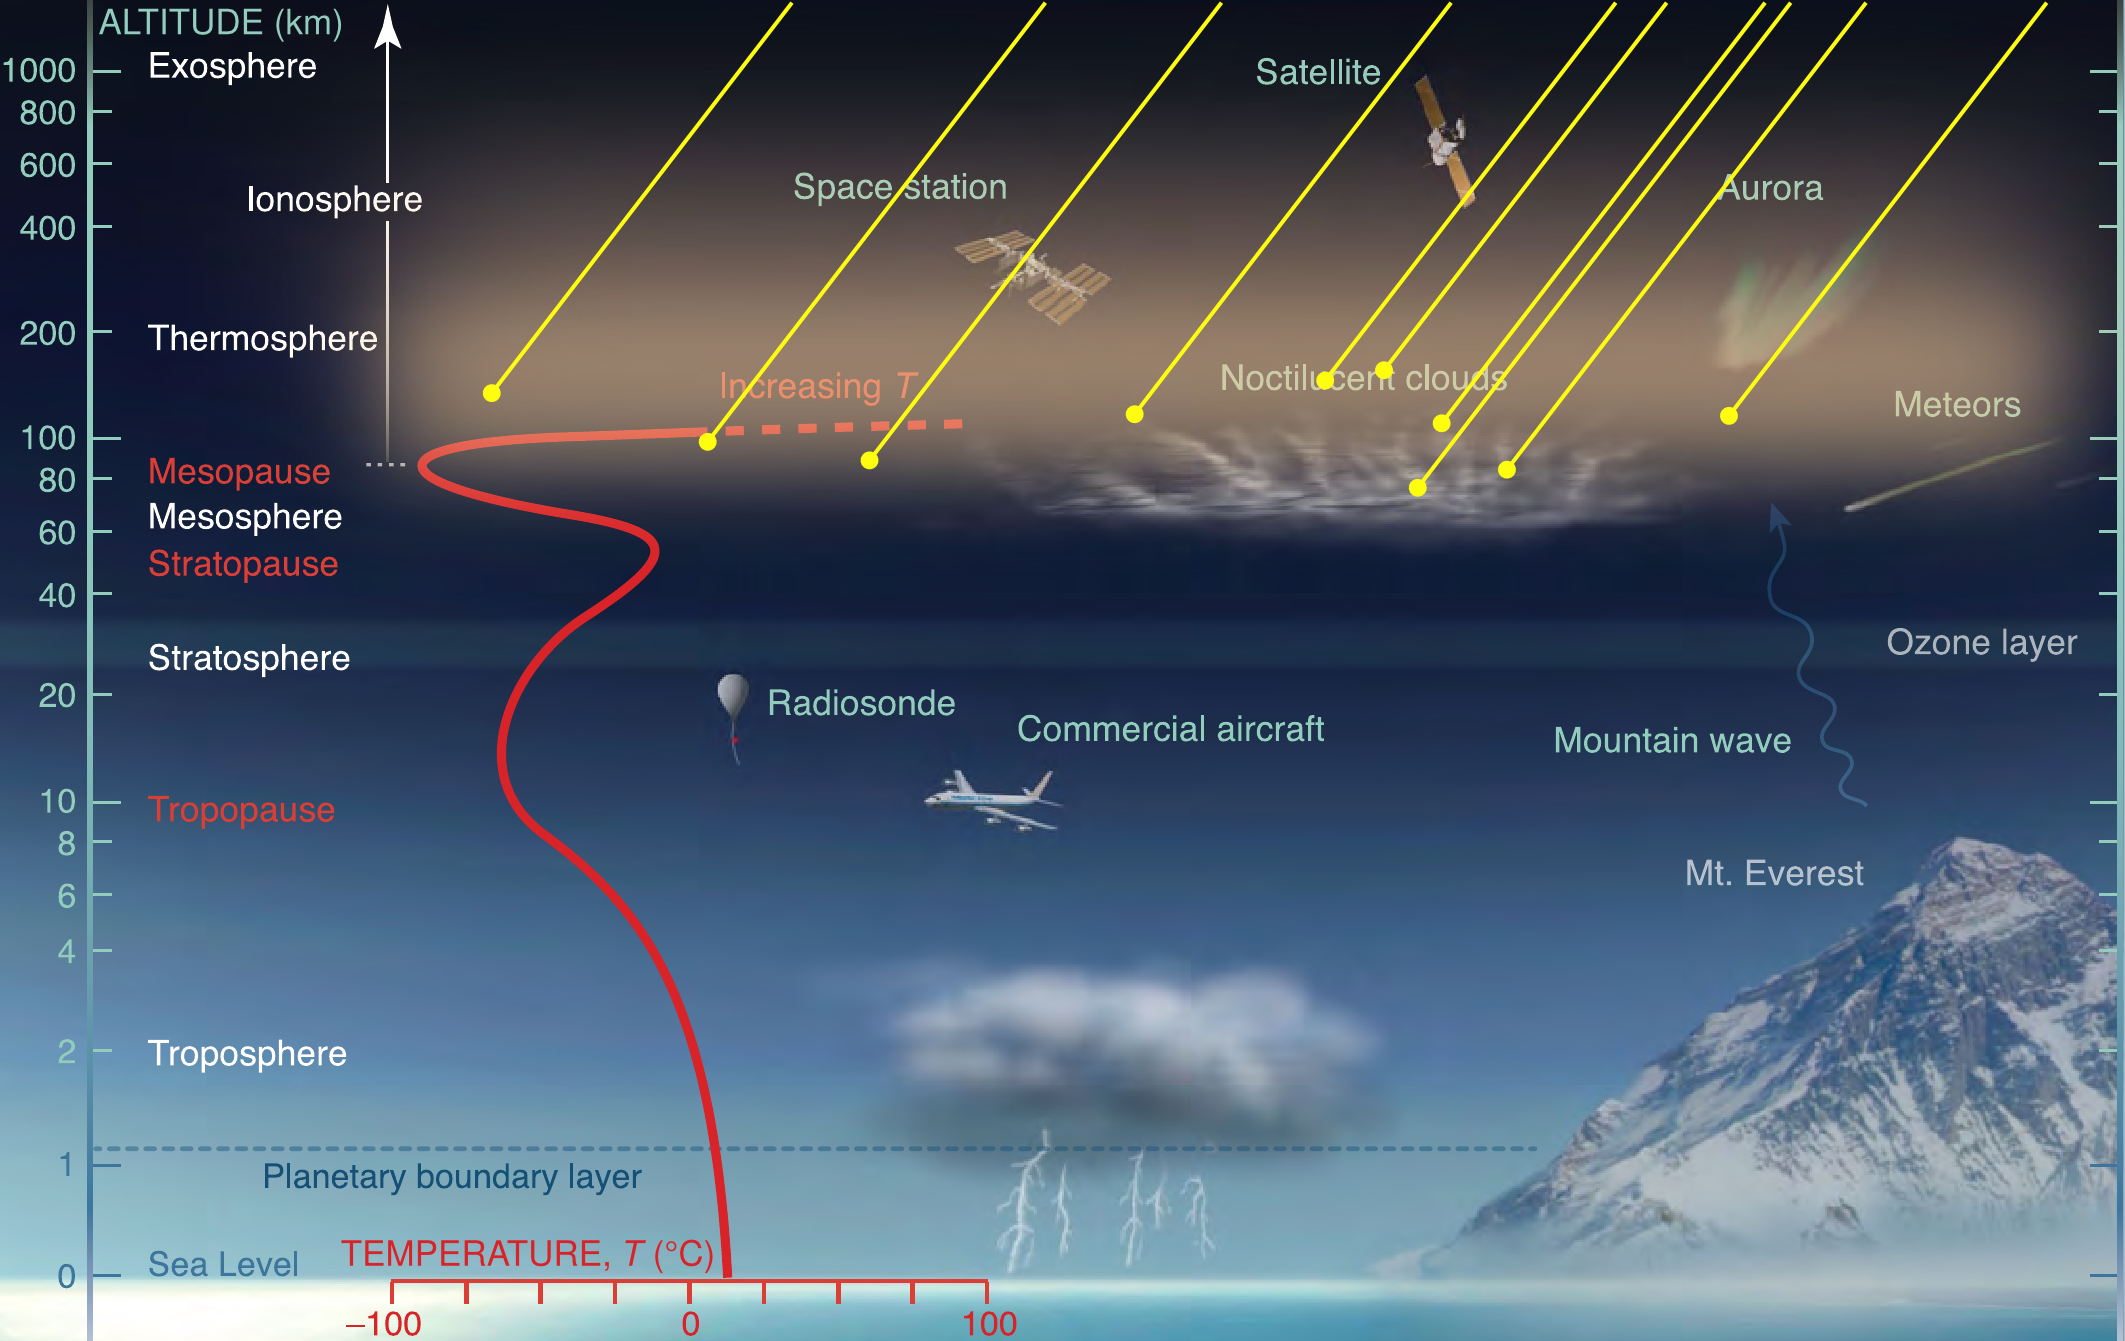
\includegraphics[width=\textwidth]{atmospheric_regions_with_radiation}
 \begin{flushright}
  \tiny
  Image from NSF (2011), CEDAR: The New Dimension
 \end{flushright}
  
 \begin{textblock}{0.47}(0.25,0.41)
  \begin{definition}
   The \alert{ionosphere} is a region of \alert{partially ionized gas (plasma)} that envelops the Earth from an altitude of about 60 km and higher.
  \end{definition}
  \vspace{-1ex}
  \begin{block}{Mechanism}
   Ionization is principally caused by solar radiation.
  \end{block}
 \end{textblock}
\end{frame}

\begin{frame}{Importance of the ionosphere}{Communications}
 \centering
 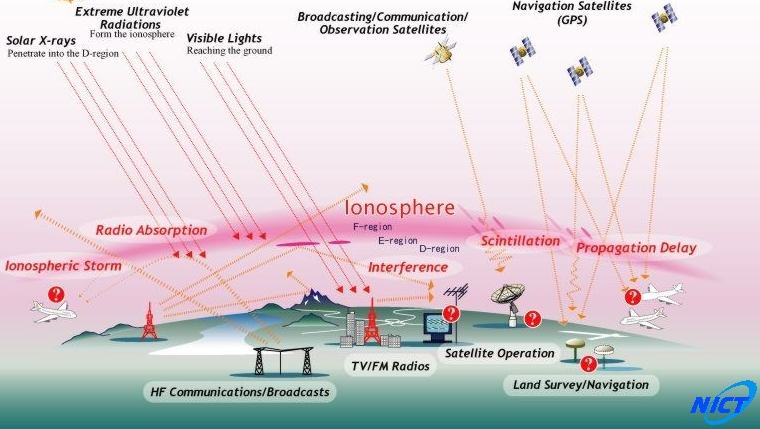
\includegraphics[width=0.7\textwidth]{ionosphere_communications}
 \begin{itemize}
  \item Radio waves of lower frequency (less than $\approx 10$\ MHz) reflect off ionosphere.
  \item Microwave frequencies (e.g. GPS) can pass through, but experience frequency-dependent refraction and delay.
  \item Plasma irregularities additionally perturb signals.
 \end{itemize}
\end{frame}

\begin{frame}{Importance of the ionosphere}{Science of the geospace system}
 \centering
 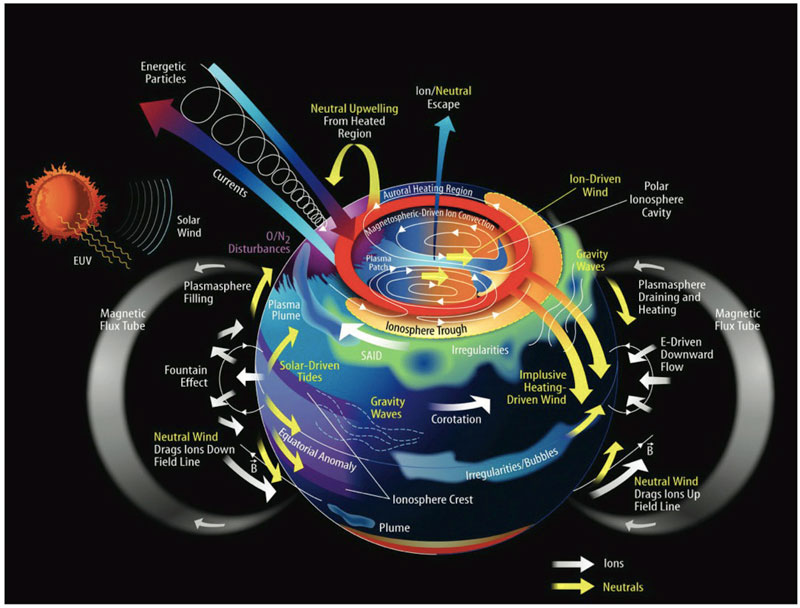
\includegraphics[height=0.8\textheight]{ionosphereprocesses}
\end{frame}

\begin{frame}{Ionospheric environment: meteoroids and meteors}
 \begin{columns}
  \column{0.5\textwidth}
  \begin{definition}[Meteoroid]
   \begin{itemize}
    \item Solid body in space
    \item Small (< 1 m in diameter)
    \item Fast (from 11 to 72 \alert{km/s})
    \item Exponentially more common as size decreases
   \end{itemize}
  \end{definition}
  \begin{columns}[onlytextwidth]
   \column{0.35\textwidth}
   \begin{beamercolorbox}{example text}
    \centering
    Micro\-meteorites\\
    (landed on Earth)
   \end{beamercolorbox}
   \column{0.65\textwidth}
   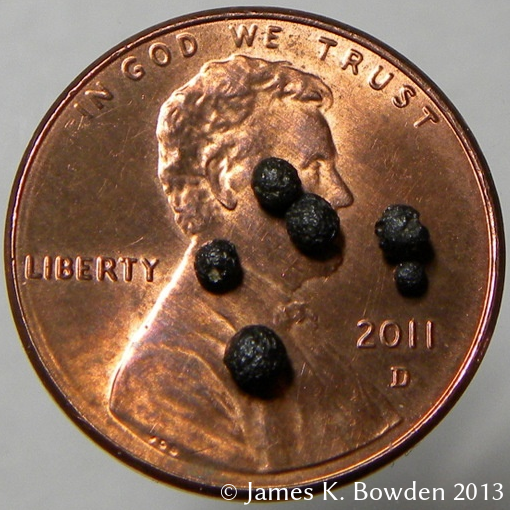
\includegraphics[width=\textwidth]{micrometeorites}
  \end{columns}
  \column{0.5\textwidth}
  \begin{definition}[Meteor]
   Plasma created by meteoroid entering the atmosphere.
  \end{definition}
  \raggedleft
  \movie[autostart,loop,width=2.1in,height=1.4in]{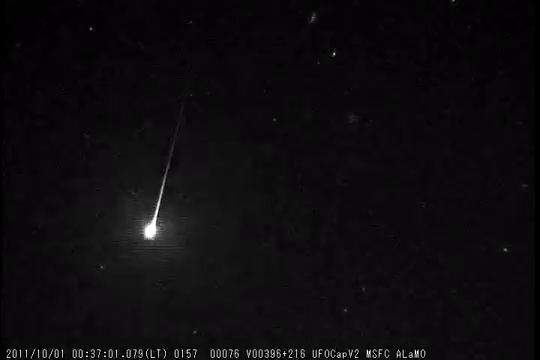
\includegraphics[width=2.1in]{meteor_spectacular_double_shot}}{movies/meteor_spectacular_double_shot.mp4}\\
  {\tiny NASA (2011)}
 \end{columns}
\end{frame}

\begin{frame}{Importance of meteoroids}
 \begin{columns}
  \column{0.6\textwidth}
  \begin{columns}[onlytextwidth]
   \column{0.35\textwidth}
   \begin{beamercolorbox}{example text}
    \centering
    Impact damage to Space Shuttle Atlantis
   \end{beamercolorbox}
   \column{0.6\textwidth}
   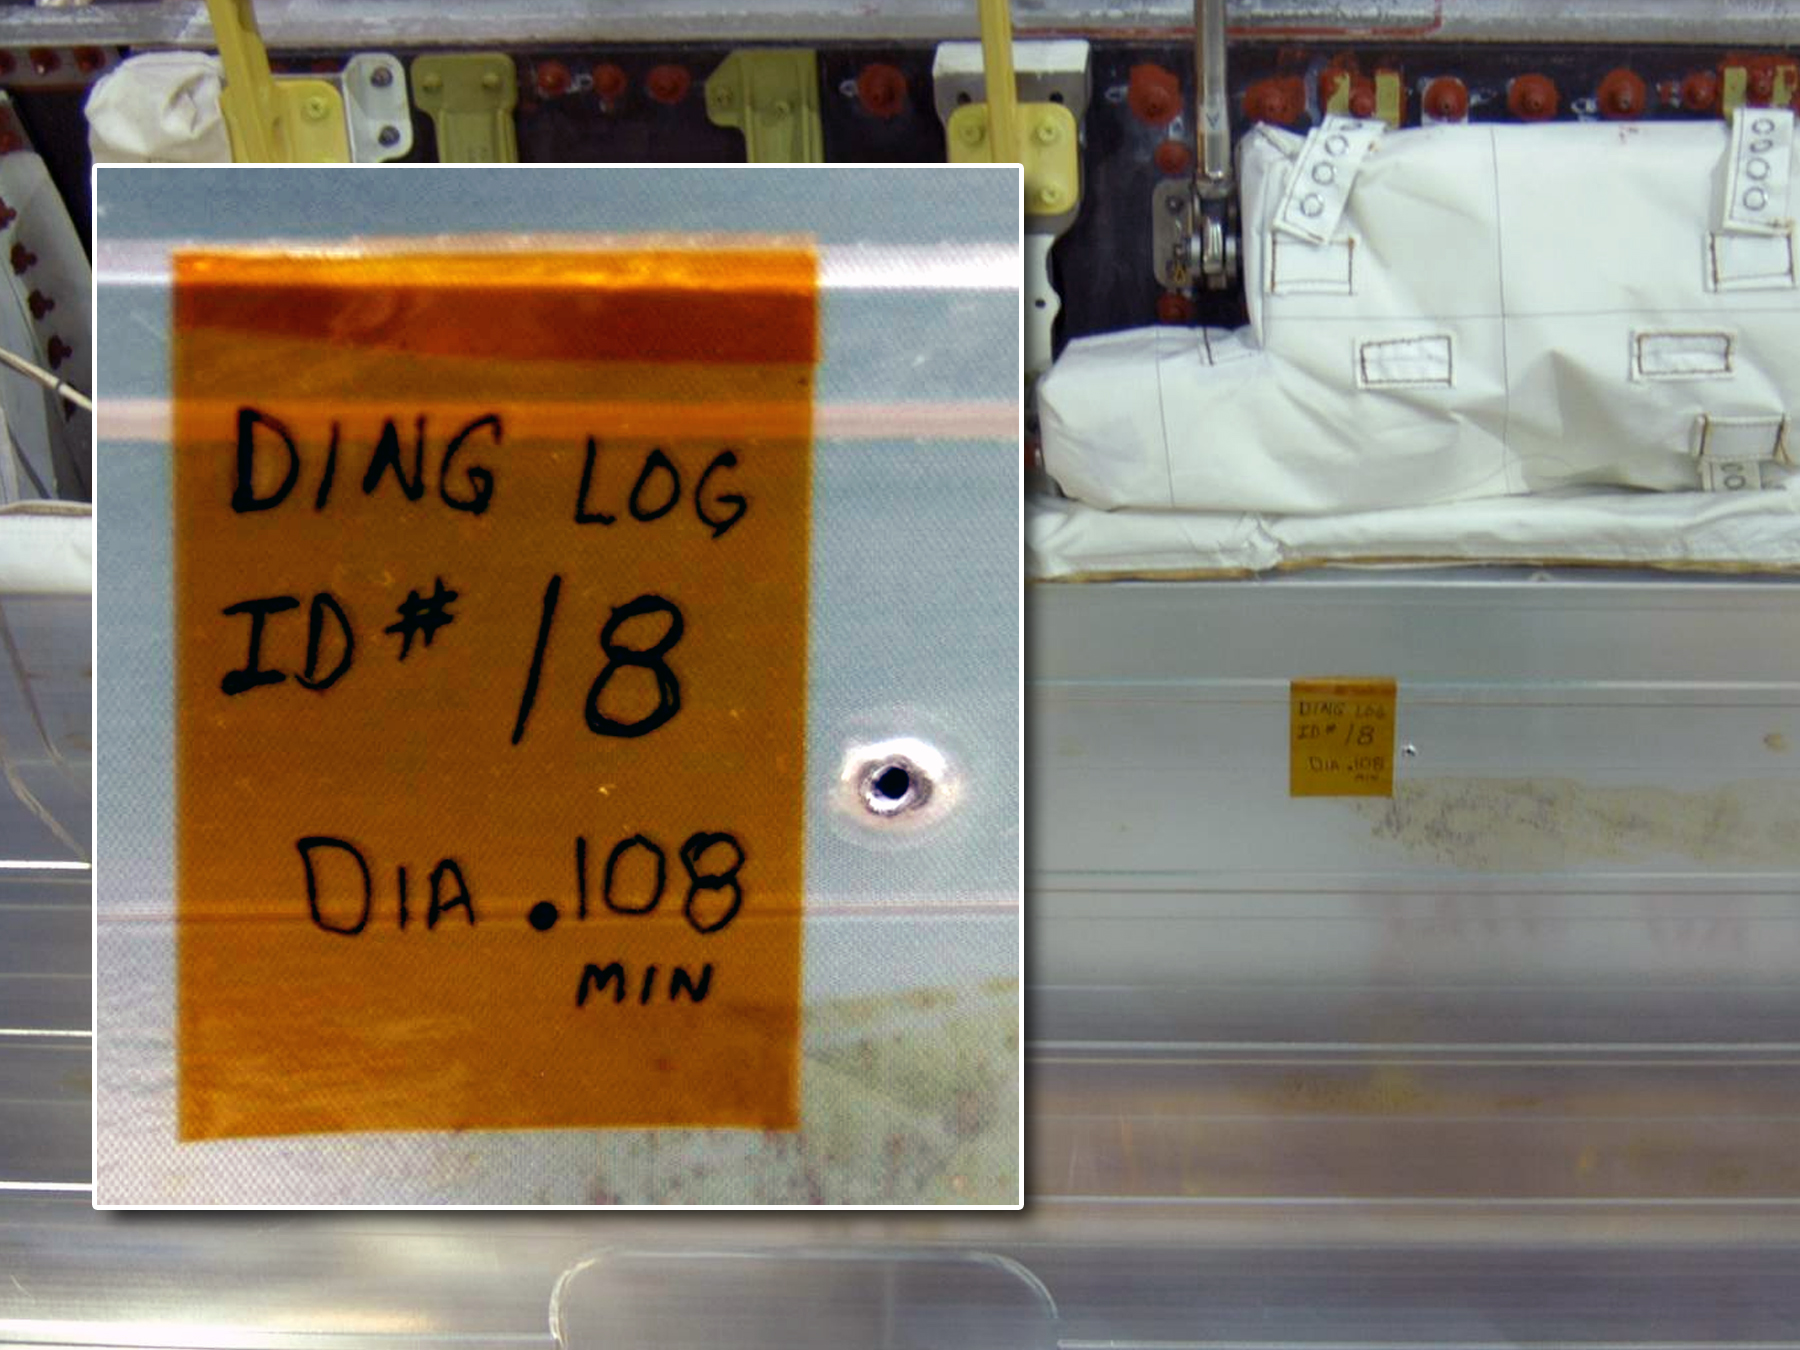
\includegraphics[width=\textwidth]{shuttle_atlantis_impact_inset}
  \end{columns}
  \begin{block}{High speed impacts}
  Threat to satellites and spacecraft from%
   \begin{itemize}
    \item mechanical damage
    \item \alert{electrical} damage
   \end{itemize}
  \end{block}
  \column{0.4\textwidth}
  \begin{block}{Required observations}
   \begin{itemize}
    \item Rate/count
    \item Size
    \item Speed
    \item Composition
   \end{itemize}
  \end{block}
 \end{columns}
 \centering
 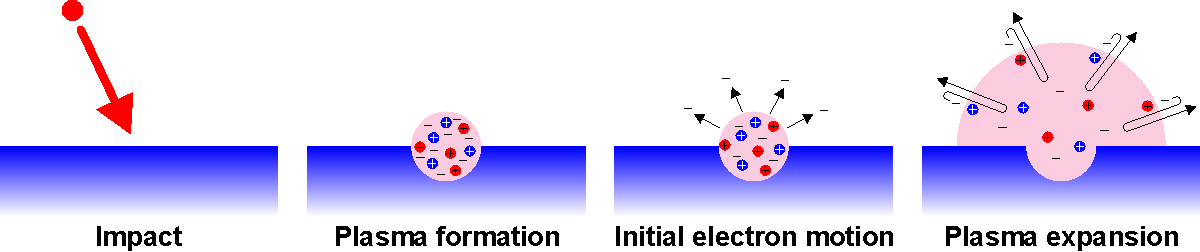
\includegraphics[width=0.75\textwidth]{ImpactPlasmaExpansion}
\end{frame}

\subsection*{Radar Measurements}

\begin{frame}{Measuring the ionosphere}
 \begin{definition}
  \alert{Incoherent Scatter Radars} (ISRs, locations shown {\color{red}below}) are radars sensitive enough to measure scattering from electrons in the background ionosphere.
 \end{definition}
 \includegraphics<1>[width=\textwidth]{isr_map}
 \includegraphics<2>[width=\textwidth]{isr_map_pfisr}
 \includegraphics<3>[width=\textwidth]{isr_map_millstone}
 \includegraphics<4>[width=\textwidth]{isr_map_jicamarca}
 
 \vspace{2ex}
 Range of ionospheric regions: \onslide<2>{polar,} \onslide<3>{mid-latitude,} \onslide<4>{equatorial.}
 \begin{textblock}{0.5}(0.25,0.525)
  \only<2>{
  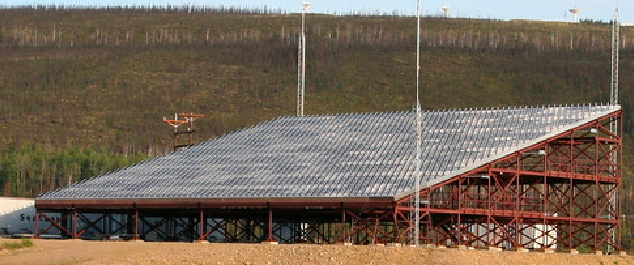
\includegraphics[height=3.6cm]{pfisr}\\
  \vspace{-3.6cm}{\color{white}\ \textbf{PFISR}}
  }
 \end{textblock}
 \begin{textblock}{0.5}(0.425,0.42)
  \only<3>{
  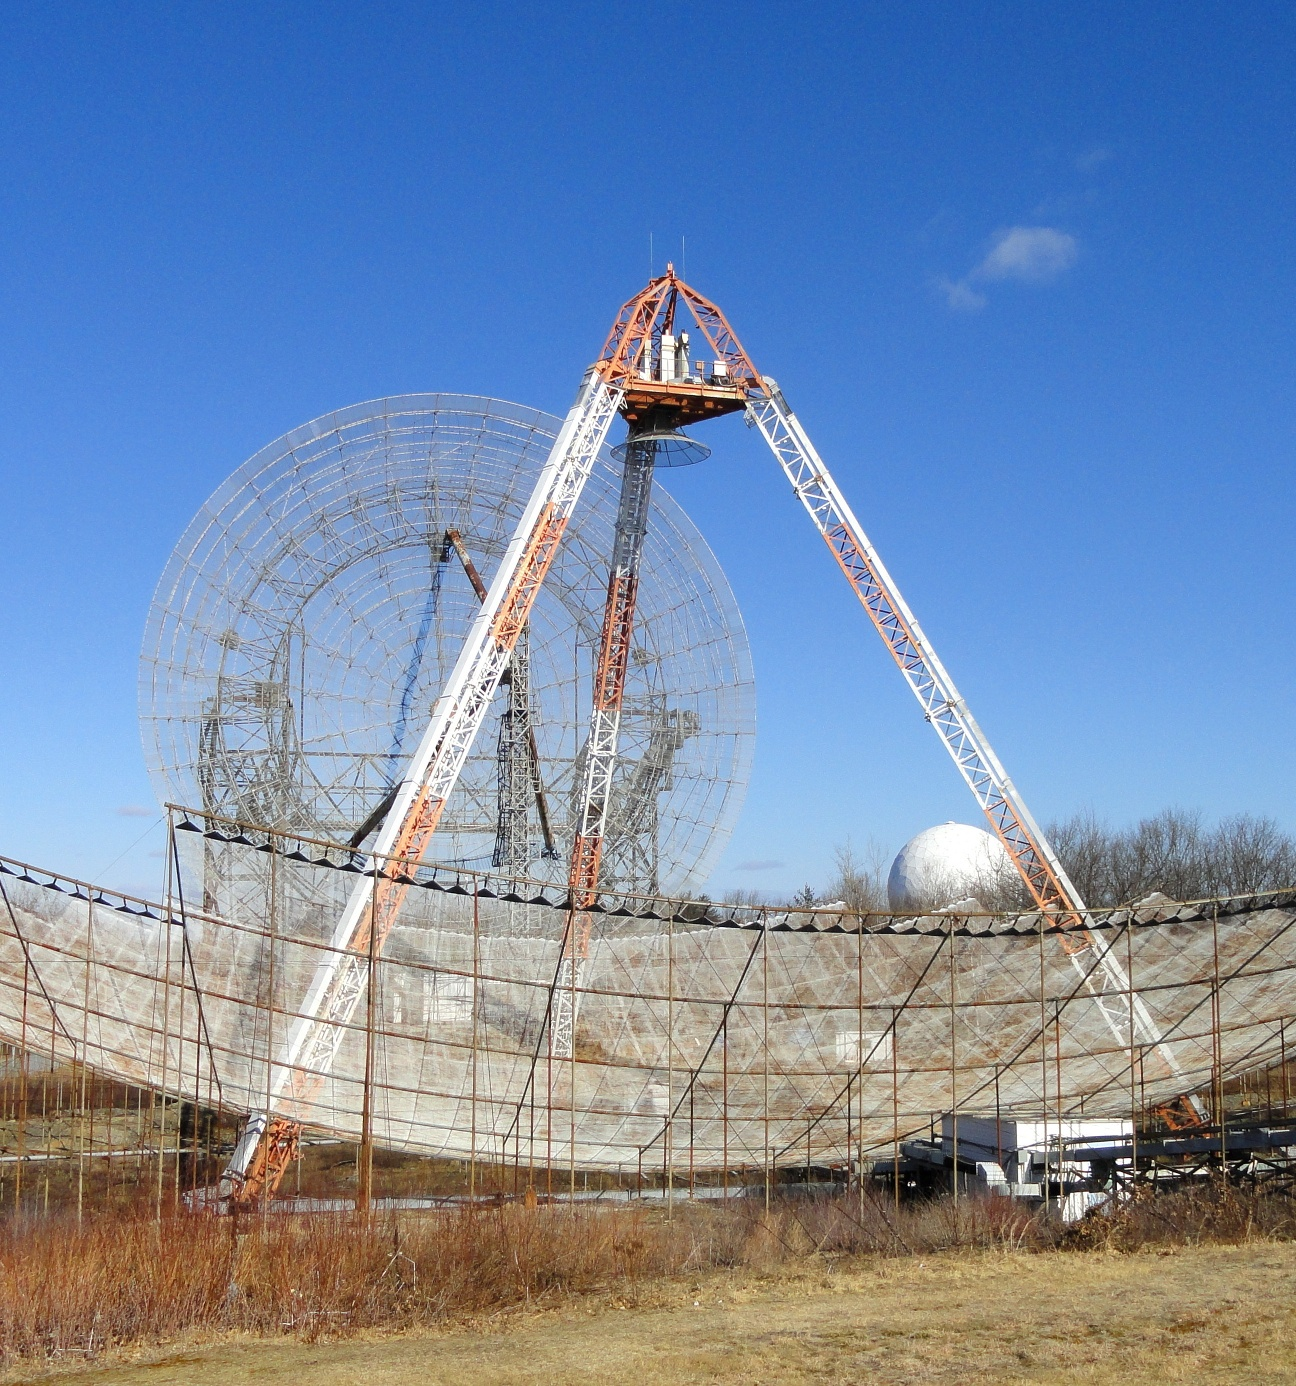
\includegraphics[height=4.75cm]{millstone_hill_radar}\\
  \vspace{-4.75cm}\ \textbf{Millstone Hill}
  }
 \end{textblock}
 \begin{textblock}{0.5}(0.425,0.525)
  \only<4>{
  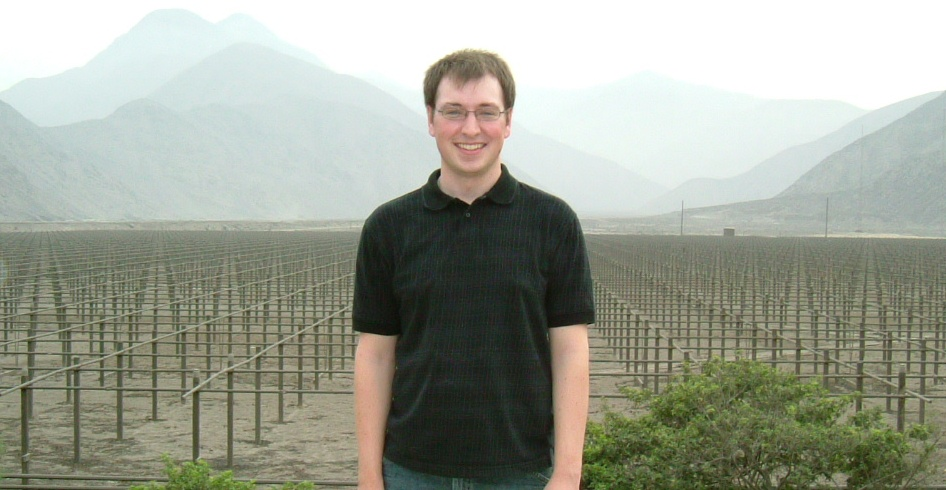
\includegraphics[height=3.6cm]{jicamarca_and_me}\\
  \vspace{-3.6cm}\ \textbf{Jicamarca}
  }
 \end{textblock}
\end{frame}

\begin{frame}{Radar meteors}
 \begin{block}{Types of scattering}
  \begin{itemize}
   \item {\color{green!80!black}Head}: ball of plasma surrounding the meteoroid
   \item {\color{purple}Trail}: plasma left in wake of meteoroid
  \end{itemize}
 \end{block}
 \centering
 \begin{tikzpicture}[thick,scale=1.175]
  \node[above right] at (0,0) {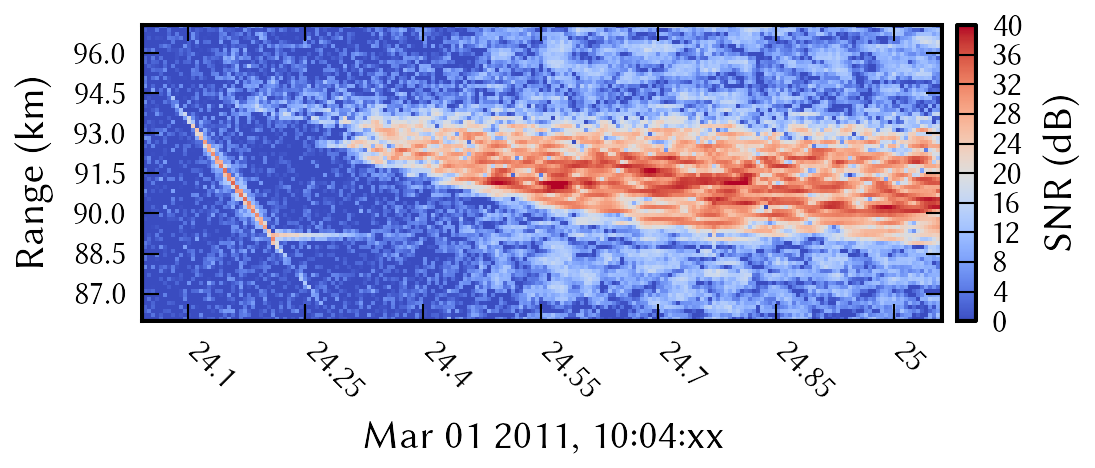
\includegraphics[scale=1.175]{head_and_flare_mf_rti_3}};
  \draw[purple] (2.8,2) rectangle (8.2,3.25);
  \draw[green!80!black,shift={(2.2,2.45)},rotate=-55] (-1.2,-0.15) rectangle (1.2,0.15);
 \end{tikzpicture}
\end{frame}

\begin{frame}{Variety of ionospheric plasma}
 There are many different plasma phenomena, each presenting its own challenges for observation.
 \makebox[\textwidth][c]{\begin{tikzpicture}[thick]
  \node[above right,image] at (0,0) {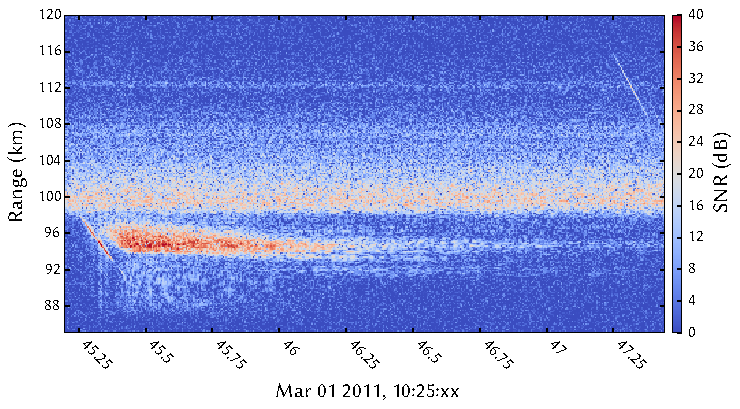
\includegraphics{equatorial_example_mf_rti_3}};
  \draw[green!80!black] (1.1,3.225) rectangle (11.36,3.9);
  \draw[purple] (1.4,2.4) rectangle (9.5,3.175);
  \draw[purple] (10.3,4.8) rectangle (11.2,6.1);
 \end{tikzpicture}}
 \begin{textblock}{0.3}(0.125,0.28)
  \begin{example}{Equatorial ionosphere}
   \begin{itemize}
    \item {\color{green!80!black}Electrojet}
    \item {\color{purple}Meteor}
   \end{itemize}
  \end{example}
 \end{textblock}
\end{frame}

\begin{frame}{At the limit: meteors}
 \makebox[\textwidth][c]{Scientific progress is limited by current signal processing techniques!}
 \vspace{1ex}
 \begin{columns}
  \column{0.25\textwidth}
  \begin{beamercolorbox}{example text}
   Fragmentation
  \end{beamercolorbox}
  \column{0.75\textwidth}
  \raggedleft
  {\tiny Mathews, et al. (2010), \emph{Geophysical Research Letters}}
  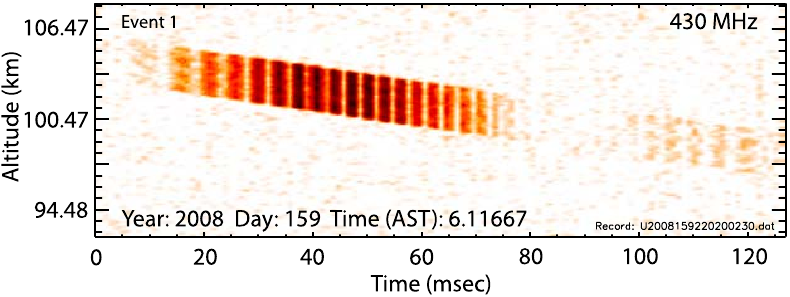
\includegraphics[width=\textwidth]{mathews_fragmentation}
 \end{columns}
 
 \begin{columns}
  \column{0.25\textwidth}
  \begin{beamercolorbox}{example text}
   Flares and terminal events
  \end{beamercolorbox}
  \column{0.75\textwidth}
  \centering
  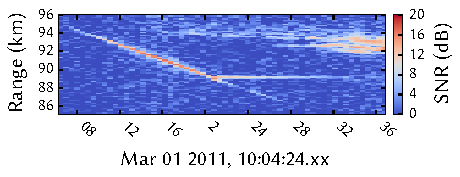
\includegraphics{flare_mf_rti_3}
 \end{columns}
\end{frame}

\begin{frame}{Measurement challenges}
 \begin{columns}
  \column{0.5\textwidth}
  \begin{enumerate}
   \item \alert{Differentiation} in a crowded and variable environment\\
   (e.g. meteors and electrojet)
   \item \alert{Self-interference} of range-spread targets\\
   (e.g. meteor trails)
   \item \alert{High resolution} to observe small-scale processes\\
   (e.g. meteoroid\\fragmentation and flares)
   \item \alert{Flexibility} to achieve all of the above at once
  \end{enumerate}
 \column{0.5\textwidth}
 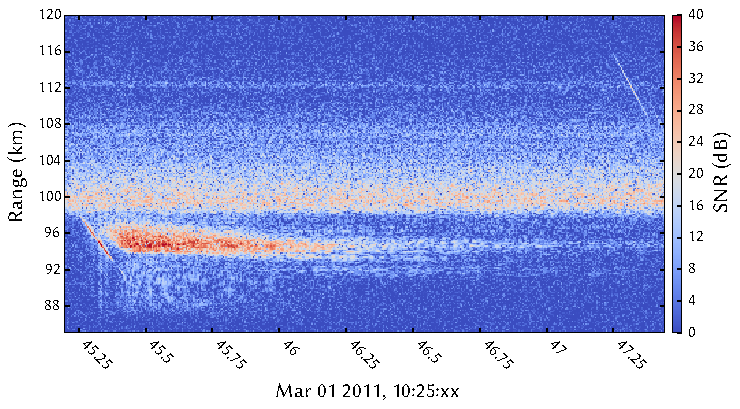
\includegraphics[width=\textwidth]{equatorial_example_mf_rti_3}\\
 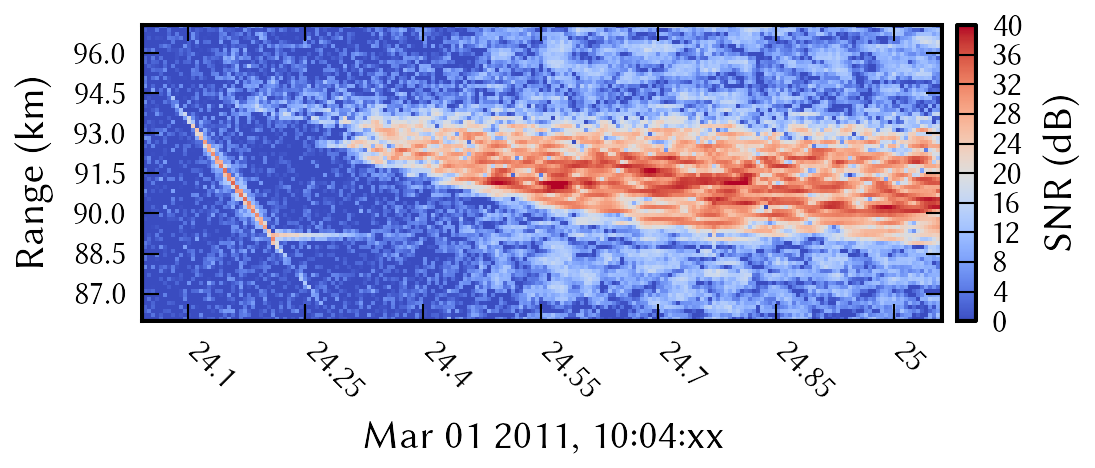
\includegraphics[width=\textwidth]{head_and_flare_mf_rti_3}\\
 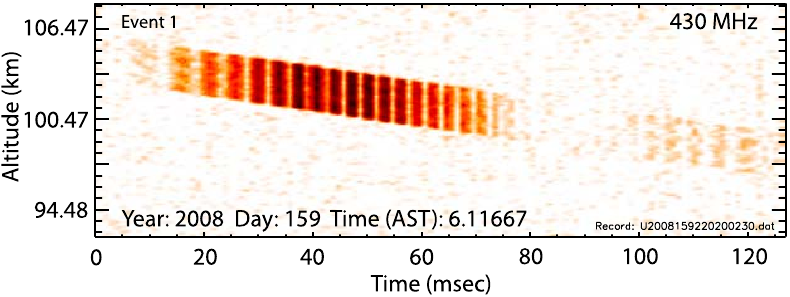
\includegraphics[width=\textwidth]{mathews_fragmentation}
 \end{columns}
\end{frame}

\subsection*{Sparsity}

\begin{frame}{A way forward: sparsity}
 Radar targets are typically sparse in range and frequency!
 \begin{center}
  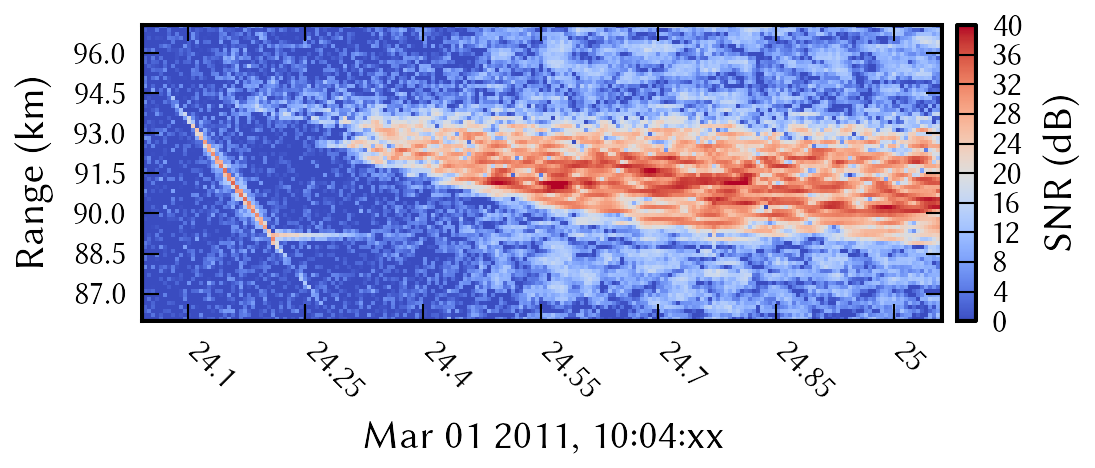
\includegraphics{head_and_flare_mf_rti_3}
 \end{center}
 \begin{center}
  \begin{minipage}{0.7\textwidth}
   \begin{alertblock}{}
    \centering
    Can use sparsity to systematically improve the quality of radar measurements.
   \end{alertblock}
  \end{minipage}
 \end{center}
\end{frame}

\begin{frame}{The world is sparse}
 \begin{definition}
  \vspace{-0.5ex}
  \begin{itemize}
   \item A vector is \alert{sparse} if only a few of its elements are nonzero.
   \item Additionally, the term is often applied loosely to when this is approximately true (i.e. most of the elements close to zero).
  \end{itemize}
  \vspace{-0.5ex}
 \end{definition}
 \begin{columns}
  \column{0.5\textwidth}
  Many natural phenomena have sparse representations:
  \begin{itemize}
   \item Music and speech (mp3)
   \item Images (jpeg)
  \end{itemize}
  \begin{exampleblock}{Alpacas (right): 8.5x savings}
   \begin{tabular}{rr}
    Uncompressed: & 3600 KB\\
    Compressed: & 420 KB
   \end{tabular}
  \end{exampleblock}
  \column{0.5\textwidth}
  \centering
  {\tiny Alpacas at the Jicamarca radar site}
  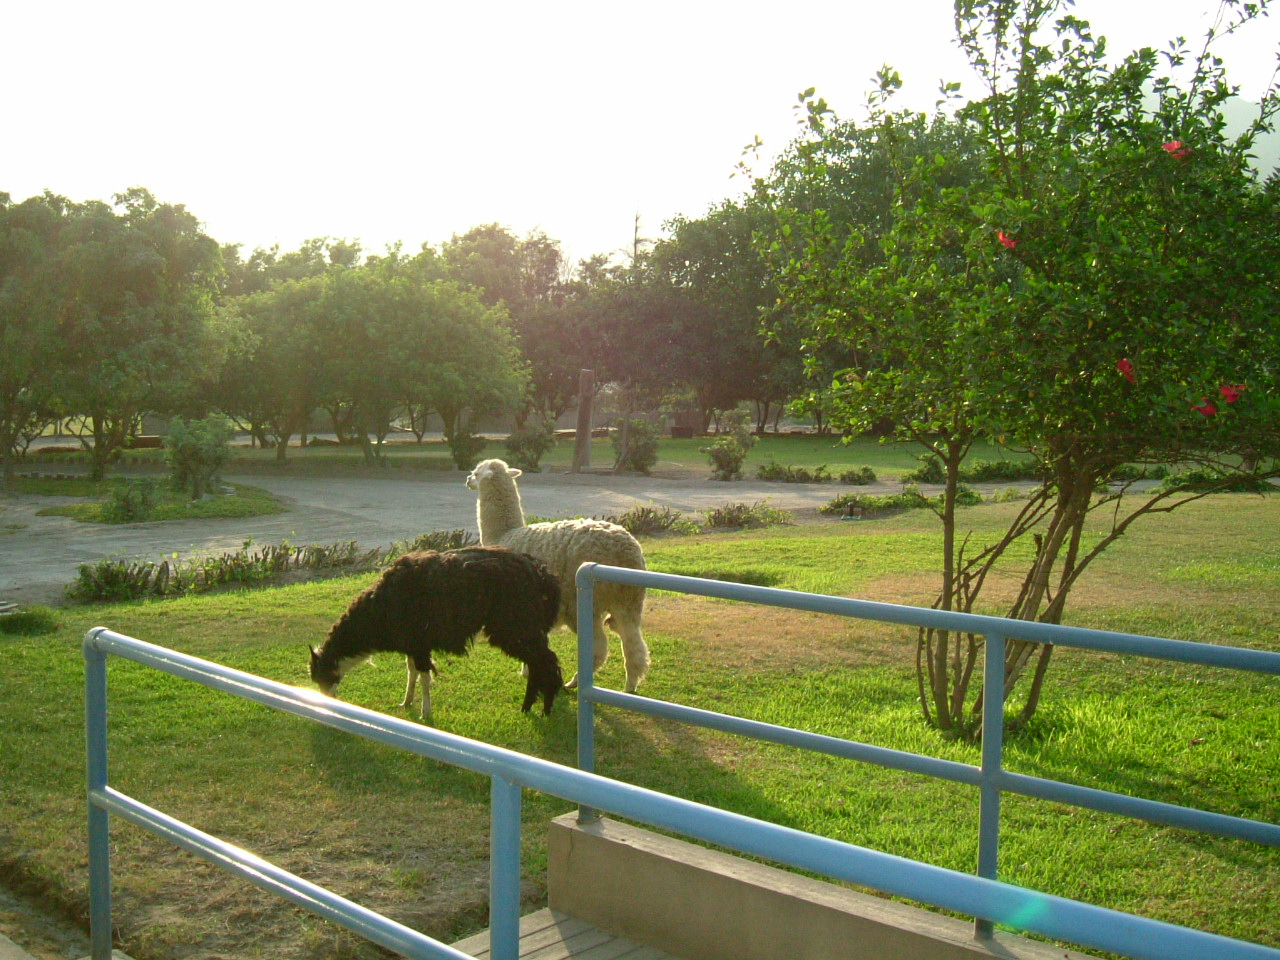
\includegraphics[width=\textwidth]{jicamarca_alpacas}
 \end{columns}
\end{frame}

\begin{frame}{Sparsity revolution}
 Exploitation of inherent signal sparsity through compressed sensing is leading to advancements in many subjects.
 \begin{columns}
  \column{0.475\textwidth}
  \begin{exampleblock}{Single pixel camera (1)}
   Smaller, cheaper, more flexible\\
   {\tiny dsp.rice.edu/cscamera}
  \end{exampleblock}
  \begin{exampleblock}{MRI (2)}
   Faster scans, higher resolution\\
   {\tiny eecs.berkeley.edu/~mlustig/CS.html}
  \end{exampleblock}
  \begin{exampleblock}{Genomics}
   High-throughput screening\\
   {\tiny erlichlab.wi.mit.edu}
  \end{exampleblock}
  \column{0.525\textwidth}
  \begin{columns}
   \column{0.05\textwidth}
   (1)
   \column{0.95\textwidth}
   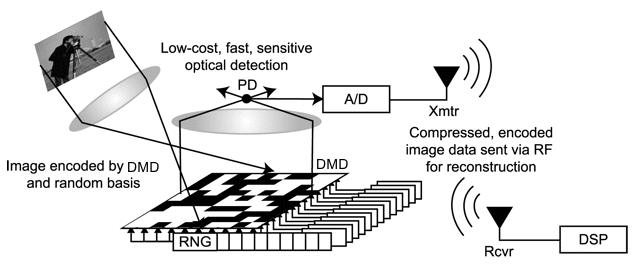
\includegraphics[width=\textwidth]{cscam}
  \end{columns}
  \vspace{2ex}
  \begin{columns}
   \column{0.05\textwidth}
   (2)
   \column{0.95\textwidth}
   \begin{minipage}[c]{0.33\textwidth}
    \scriptsize\centering
    Original
   \end{minipage}%
   \begin{minipage}[c]{0.33\textwidth}
    \scriptsize\centering
    Filtered backprojection
   \end{minipage}%
   \begin{minipage}[c]{0.33\textwidth}
    \scriptsize\centering
    Compressed sensing
   \end{minipage}
   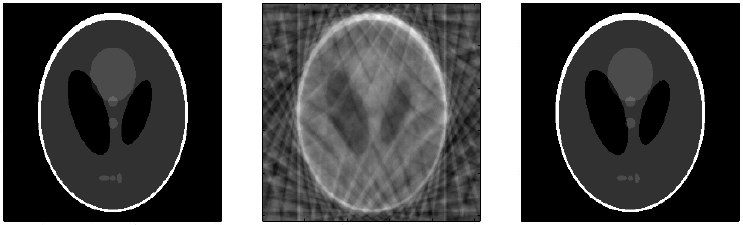
\includegraphics[width=\textwidth]{mri_cs}
  \end{columns}
 \end{columns}
\end{frame}

\subsection*{}

\begin{frame}<1-6>[label=contributions]{Contributions}
 In order to enable \alert{flexible high-resolution measurements} of ionospheric plasma phenomena, including interfering and range-spread targets, I made the following contributions:
 \begin{enumerate}
  \item<2,8-> Derived a discrete \alert{radar model} that captures signal sparsity in delay-frequency space.
  \item<3,9-> Uncovered the adjoint relationship between the model and existing matched filter techniques, resulting in an \alert{intuitive interpretation} of the waveform inversion process.
  \item<4,10-> \alert{Analyzed the model} to show how it exactly represents off-grid and distributed scatterers and preserves their sparsity.
  \item<5,11-> Created and tuned an \alert{efficient implementation} of waveform inversion using modern convex optimization techniques.
  \item<6,12-> \alert{Demonstrated the flexibility and effectiveness} of the inversion technique by removing filtering artifacts from meteor observations made with a variety of radar waveforms.
 \end{enumerate}
\end{frame}

\begin{frame}{Additional contributions}
 In addition, I also made the following contributions that will not be covered in this talk:
 \begin{enumerate}
  \item Created a \alert{range-time-frequency clustering algorithm} for detection and classification of ionospheric radar signals.
  \item Simulated the statistical accuracy of interpolated matched filter estimation for range and range-rate \alert{super-resolution of meteor head echoes}.
 \end{enumerate}
\end{frame}

\begin{frame}{Outline}
 \tableofcontents[hideallsubsections]
\end{frame}

\section{Radar Background}
\subsection{Pulse Encoding/Decoding}

\begin{frame}{Radar pulse length}
 \begin{columns}
  \column{0.5\textwidth}
  \begin{block}{Short pulse}
   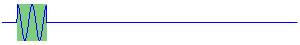
\includegraphics[width=\textwidth]{shortpulse}
   \begin{itemize}
    \item Low range ambiguity
    \item Simple to interpret
   \end{itemize}
  \end{block}
  \column{0.5\textwidth}
  \begin{block}{Long pulse}
   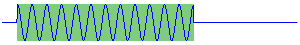
\includegraphics[width=\textwidth]{longpulse}
   \begin{itemize}
    \item Fine frequency resolution
    \item High total power
   \end{itemize}
  \end{block}
 \end{columns}
 \vspace{2ex}
 Some objectives favor a shorter radar pulse, while others favor a longer radar pulse.
\end{frame}

\begin{frame}{Coded pulses}
 \begin{itemize}
  \item Encoding allows long pulses to have the low range ambiguity of short pulses.
  \item One method: divide pulse into \alert{bauds} of constant phase.
 \end{itemize}
 \begin{exampleblock}{Barker-13 code}
  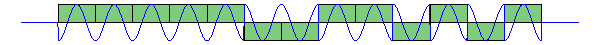
\includegraphics[width=\textwidth]{barker13pulse}
 \end{exampleblock}
 \begin{exampleblock}{Minimum peak sidelobe code}
  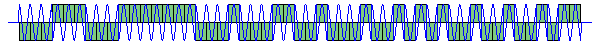
\includegraphics[width=\textwidth]{mslpulse}
 \end{exampleblock}
 \begin{exampleblock}{Linear frequency modulation (LFM chirp)}
  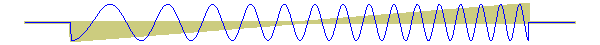
\includegraphics[width=\textwidth]{lfmpulse}
 \end{exampleblock}
\end{frame}

\begin{frame}{The matched filter}
 \begin{definition}
  The \alert{matched filter} correlates every segment of the received signal with the transmitted pulse.
 \end{definition}
 It produces a peak at the target's range (delay), achieving a rough form of decoding with ambiguous \alert{sidelobes}.
 \begin{example}[Barker-13 code, Minimum sidelobe code]
 \end{example}
 \centering
 \movie[autostart,loop,width=4in,height=1.501730in]{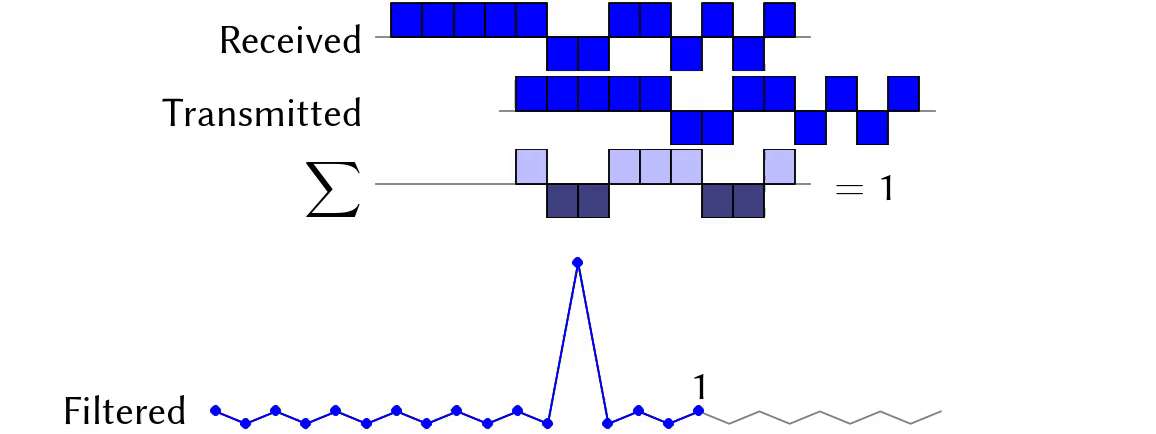
\includegraphics[width=4in]{autocorrelation_animation_b13_msl}}{movies/autocorrelation_animation_b13_msl.mp4}
\end{frame}

\begin{frame}{Frequency filter banks}
 \begin{block}{Doppler frequency shift}
  If the target is moving {\color{blue}toward} or {\color{red}away from} the radar, the reflected signal is frequency shifted {\color{blue}up} or {\color{red}{down}}.
 \end{block}
 \begin{itemize}
  \item Matched filter needs to be similarly frequency shifted
  \item True frequency shift is not known ahead of time
  \item Process signal with a bank of differently-shifted filters
 \end{itemize}
 \begin{columns}
  \column{0.5\textwidth}
  \begin{beamercolorbox}{example text}
   \centering
   Result of filter bank for\\centered "point" target,\\using Barker-13 code
  \end{beamercolorbox}
  \column{0.5\textwidth}
  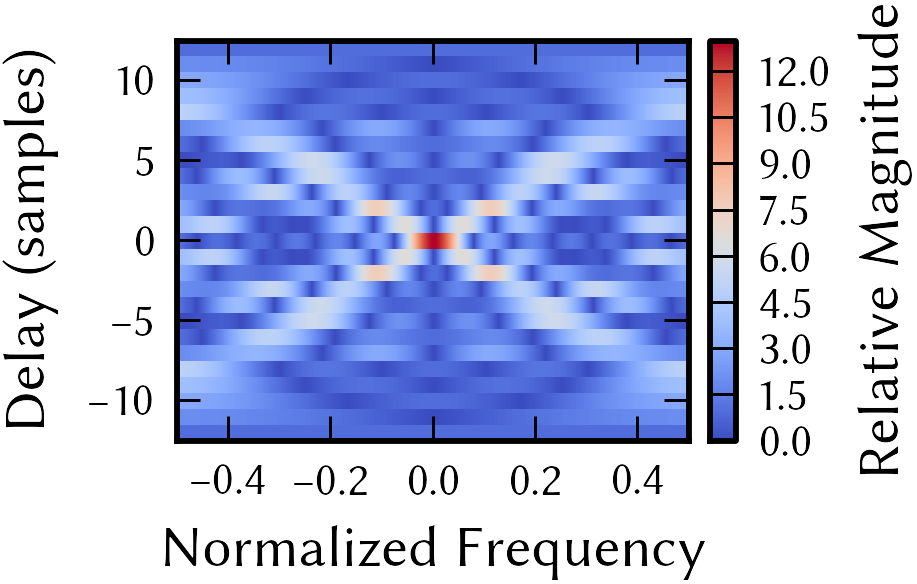
\includegraphics{ambiguity_barker13}
 \end{columns}
\end{frame}

\subsection{Measurement Ambiguity}

\begin{frame}{Ambiguity functions}
 \begin{definition}
  A delay-frequency \alert{ambiguity function} is produced when a signal is matched against itself using a filter bank.
 \end{definition}
 \begin{columns}
  \column{0.5\textwidth}
  \centering
  Uncoded pulse\\
  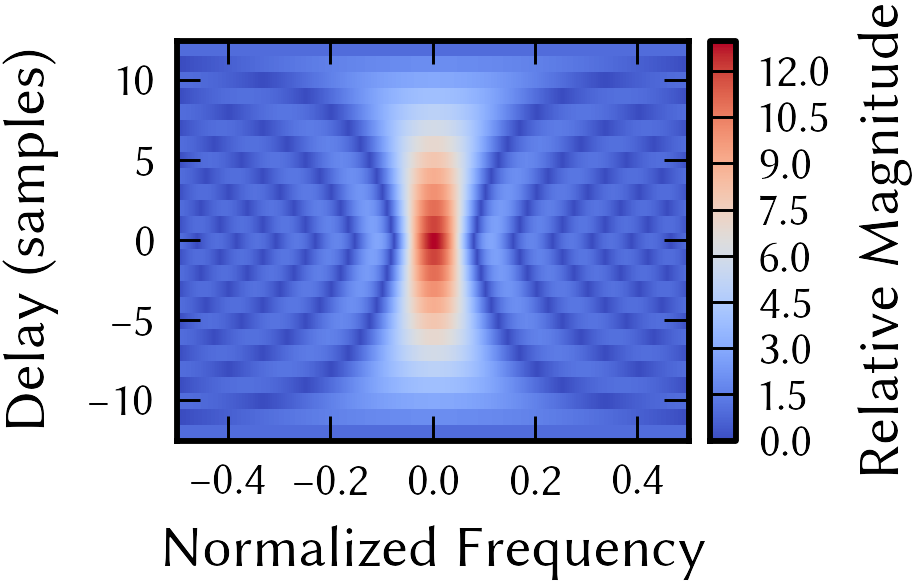
\includegraphics{ambiguity_uncoded}
  \column{0.5\textwidth}
  \centering
  Barker-13\\
  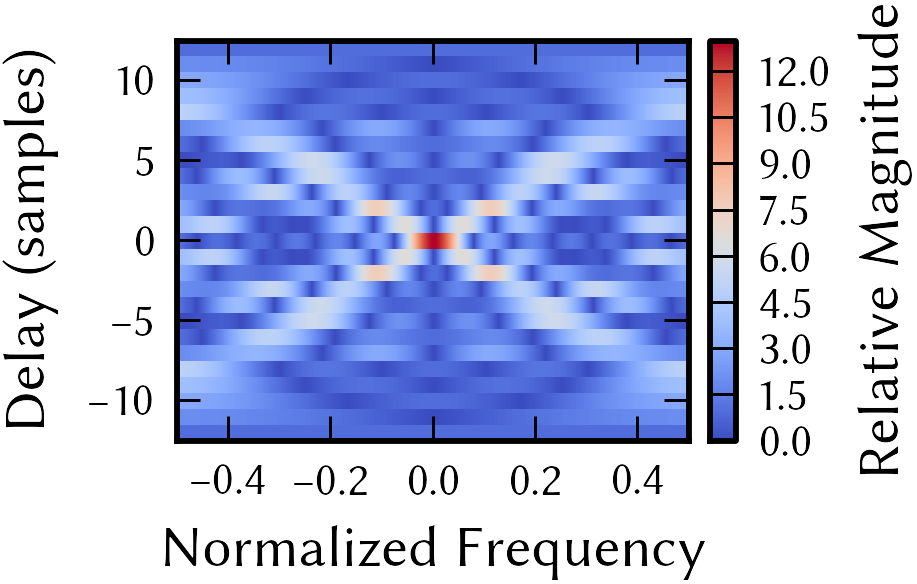
\includegraphics{ambiguity_barker13}
 \end{columns}
 \begin{alertblock}{}
  The ambiguity function describes the delay-frequency sidelobes of a code.
 \end{alertblock}
\end{frame}

\begin{frame}{More example ambiguity functions}
 \begin{columns}
  \column{0.5\textwidth}
  \centering
  Minimum sidelobe\\
  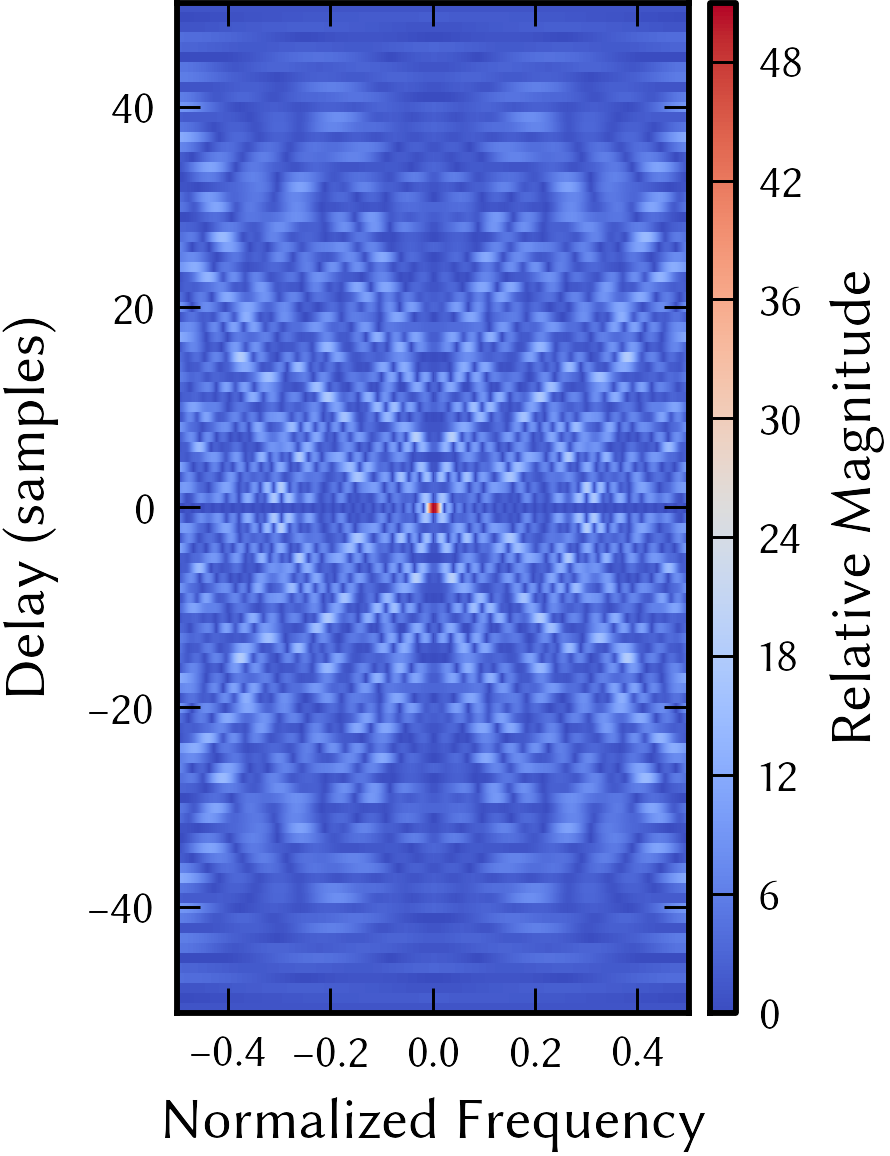
\includegraphics{ambiguity_msl}
  \column{0.5\textwidth}
  \centering
  LFM Chirp\\
  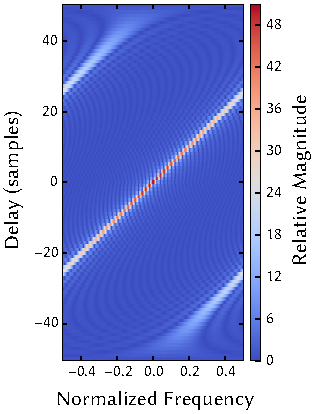
\includegraphics{ambiguity_lfm}
 \end{columns}
\end{frame}

\begin{frame}{Range sidelobes in action}
 Range sidelobes dominate the output of uncoded measurements, while coded pulses are better but still noticeably corrupted.
 \begin{tikzpicture}
  \tikzstyle{every node}=[minimum width=\widthof{Near-ideal}+2ex]
  \node[left,align=center] at (0,0.5) {Uncoded};
  \node[right,image] at (0,0) {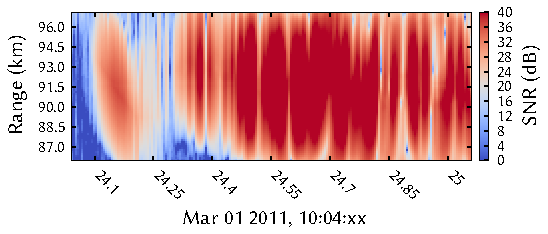
\includegraphics{head_and_flare_mf_rti_2}};
  \fill[white] (0,-1.125) rectangle (9,-0.875);
  \node[left,align=center] at (0,-2.3) {Minimum\\sidelobe\\code};
  \node[right,image] at (0,-2.8) {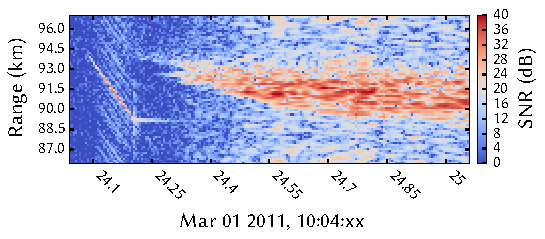
\includegraphics{head_and_flare_mf_rti_1}};
 \end{tikzpicture}
\end{frame}

\begin{frame}{Effect of sidelobes}
 Sidelobes (delay-frequency ambiguity) are the primary reason that outstanding ionospheric science questions cannot be satisfactorily answered.
 \vspace{1ex}
 \begin{columns}
  \column{0.25\textwidth}
  \begin{beamercolorbox}{example text}
   Fragmentation
  \end{beamercolorbox}
  \column{0.75\textwidth}
  \raggedleft
  {\tiny Mathews, et al. (2010), \emph{Geophysical Research Letters}}
  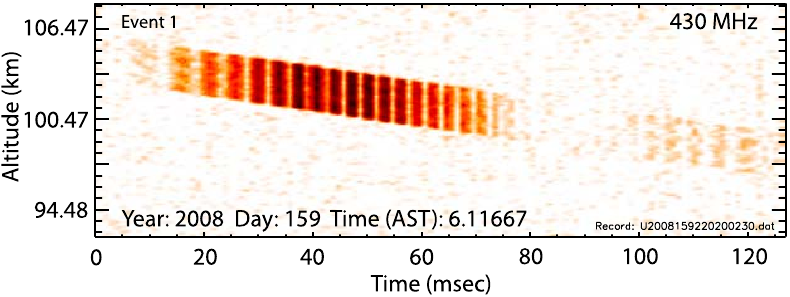
\includegraphics[width=\textwidth]{mathews_fragmentation}
 \end{columns}
 
 \begin{columns}
  \column{0.25\textwidth}
  \begin{beamercolorbox}{example text}
   Flares and terminal events
  \end{beamercolorbox}
  \column{0.75\textwidth}
  \centering
  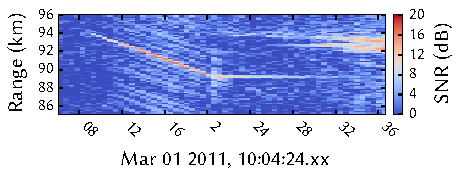
\includegraphics{flare_mf_rti_1}
 \end{columns}
\end{frame}

\begin{frame}{Goal: sidelobe removal}
 \begin{tikzpicture}
  \tikzstyle{every node}=[minimum width=\widthof{Near-ideal}+2ex]
  \node[left,align=center] at (0,0.5) {Minimum\\sidelobe\\code};
  \node[right,image] at (0,0) {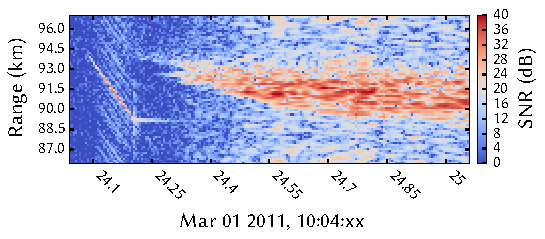
\includegraphics{head_and_flare_mf_rti_1}};
  \fill[white] (0,-1.125) rectangle (9,-0.875);
  \node[left,align=center] at (0,-2.3) {Near-ideal\\decoding};
  \node[right,image] at (0,-2.8) {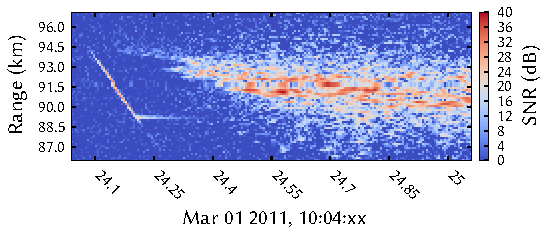
\includegraphics{head_and_flare_recovered_rti_noise_1}};
 \end{tikzpicture}
 Infinite number of ways to decode and get a target scene that reproduces the measurements!
\end{frame}

\subsection{Current Techniques}

\begin{frame}{Delay-frequency sidelobe mitigation in use}
 \begin{enumerate}
  \item Codes with good sidelobe properties
  \begin{itemize}
   \item e.g. Barker-13, minimum peak sidelobe, LFM chirp
   \item Most prevalent strategy
   \item Only effective when it is simple to \alert{ignore remaining sidelobes}
  \end{itemize}
  \item Alternating codes
  \begin{itemize}
   \item Set of codes over multiple pulses
   \item When pulses summed together, sidelobes cancel
   \item Target properties must remain stationary
  \end{itemize}
  \item Inverse filters
  \begin{itemize}
   \item Alternative to matched filter
   \item Loss of SNR depending on code
   \item Produces no range sidelobes at target's frequency shift
  \end{itemize}
 \end{enumerate}
 These strategies severely constrain the \alert{flexibility} and \alert{accuracy} of ionospheric radar measurements!
\end{frame}

\begin{frame}{Inverse filter ambiguity function}
 \begin{example}
  Ambiguity function comparison for Barker-13 code.
 \end{example}
 \begin{columns}
  \column{0.5\textwidth}
  \centering
  Matched filter\\
  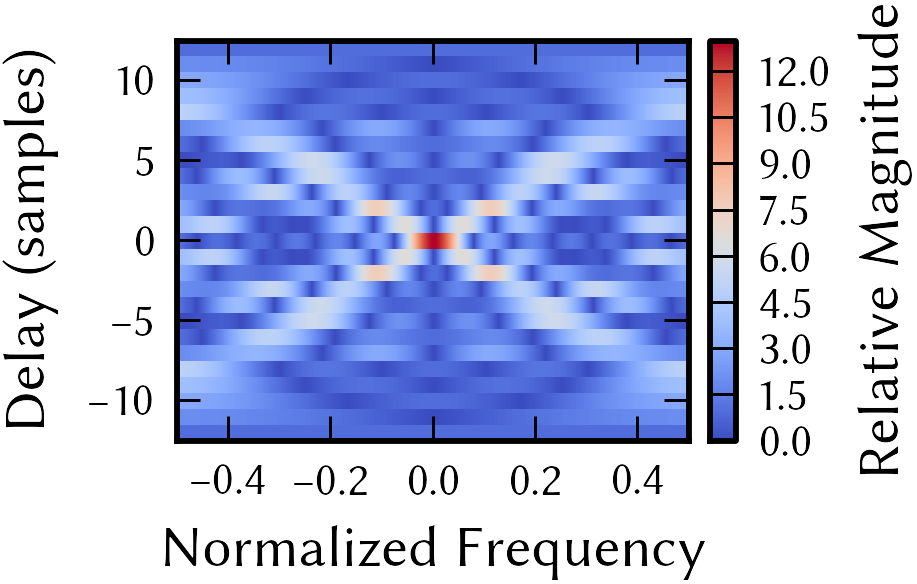
\includegraphics{ambiguity_barker13}
  \column{0.5\textwidth}
  \centering
  Inverse filter\\
  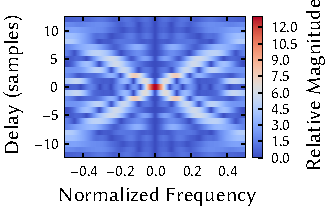
\includegraphics{inverse_ambiguity_barker13}
 \end{columns}
 \begin{alertblock}{}
  No advantage if Doppler shift is unknown or multiple frequencies must be decoded!
 \end{alertblock}
\end{frame}

\section{My Radar Model}
\subsection{Defining the Model}

\begin{frame}{Matched filtering as imaging}
 \begin{block}{Imaging analogy}
  Matched filter "image" is blurred by the ambiguity function:
  \begin{equation*}
   {\color{red}h[n,p]} * {\color{blue}\chi[n,p]} = {\color{purple}x[n,p]}
  \end{equation*}
  \vspace{-2ex}
  \begin{columns}[onlytextwidth]
   \column{0.33\textwidth}
   \centering
   {\color{red}Target reflectivity\\(source image)}
   \column{0.33\textwidth}
   \centering
   {\color{blue}Ambiguity function\\(point-spread func.)}
   \column{0.33\textwidth}
   \centering
   {\color{purple}Matched filter result\\(measured image)}
  \end{columns}
 \end{block}
 \begin{columns}[onlytextwidth]
  \column{0.33\textwidth}
  \centering
  \includegraphics<1>{blurred_image_example_orig}
  \column{0.33\textwidth}
  \centering
  \includegraphics<1>{blurred_image_example_kernel}
  \column{0.33\textwidth}
  \centering
  \includegraphics<1>{blurred_image_example_blurred}
 \end{columns}
\end{frame}

\begin{frame}{Radar model from matched filter}
 \begin{columns}
  \column{0.5\textwidth}
  \begin{block}{Ambiguity equation}
   \vspace{-4ex}\begin{align*}
    x[n,p] &= \chi[n,p] * h[n,p]\\[2ex]
    A^*\left(y[m]\right) 
    &= A^*\left(A\left(h[n,p]\right)\right)
   \end{align*}\vspace{-4ex}
  \end{block}
  \column{0.5\textwidth}
  \begin{itemize}
   \item Matched filtering is $A^*$
   \item Ambiguity function is $A^*A$
   \item Indices: \begin{tabular}{cc}
          $m$ & sample\\
          $n$ & frequency\\
          $p$ & delay
         \end{tabular}
  \end{itemize}
 \end{columns}
 \vspace{4ex}
 \begin{columns}
  \column{0.5\textwidth}
  \begin{block}{Radar model}
   Simplify by removing excess matched filtering operation:
   \begin{equation*}
    {\color{purple}y[m]} = {\color{blue}A}\left({\color{red}h[n,p]}\right)
   \end{equation*}
   \vspace{-2ex}
   \begin{columns}[onlytextwidth]
    \column{0.33\textwidth}
    \centering
    {\color{purple}Measured signal}
    \column{0.33\textwidth}
    \centering
    {\color{blue}Radar model}
    \column{0.33\textwidth}
    \centering
    {\color{red}Target reflectivity}
   \end{columns}
  \end{block}
  \column{0.5\textwidth}
  \begin{itemize}
   \item Radar model is \alert{adjoint} (conjugate transpose) of matched filter
   \item Non-invertible because under-determined
   \item Sparsity of target reflectivity is key to solution
  \end{itemize}
 \end{columns}
\end{frame}

\begin{frame}<1>{Alternative interpretation}
 \vspace{-2ex}
 \begin{columns}
  \column{0.5\textwidth}
  \begin{block}{Matched filter ($A^*$)}
   Correlates received signal with expected return from point targets with different delays and frequency shifts.
  \end{block}
  \begin{block}{Radar model ($A$)}
   Simulates received signal as \alert{sum of returns from point targets} with different delays and frequency shifts.
  \end{block}
  \column{0.5\textwidth}
  \centering
  Grid of point targets
  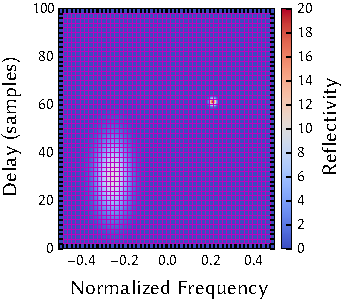
\includegraphics{range_doppler_discretization}
  \only<1>{
   \begin{equation*}
    y = A({\color{purple!70!white}h[n,p]})
   \end{equation*}
  }
 \end{columns}
 \only<2>{
 \vspace{-1ex}
  \begin{equation*}
   y[m] = \sum_{p=0}^{P-1} \frac{1}{\sqrt{N}} s[m - p + L - 1] \left(\sum_{n=0}^{N-1} e^{2\pi i n m / N} h[n,p] \right)
  \end{equation*}
 }
\end{frame}

\subsection{Representation of Targets}

\begin{frame}{Model discretization from radar signal equation}
 \begin{block}{Narrow-band radar equation for received signal}
  \vspace{-2ex}
  \begin{equation*}
   {\color{purple}y(t)} = \int_0^T \int_{-\infty}^{\infty} {\color{green!50!black}s(t - \lambda)} {\color{blue}e^{2\pi i f (t - \lambda)}} {\color{red}h(f, \lambda)} \dee{f} \dee\lambda
  \end{equation*}
  \vspace{-2ex}
 \end{block}
 \begin{columns}[onlytextwidth]
  \column{0.25\textwidth}
  \centering
  {\color{purple}Measured signal}
  \column{0.25\textwidth}
  \centering
  {\color{green!50!black}Transmitted signal}
  \column{0.25\textwidth}
  \centering
  {\color{blue}Frequency shift}
  \column{0.25\textwidth}
  \centering
  {\color{red}Target reflectivity}
 \end{columns}
 \begin{center}
  \begin{tabular}{llc}
   $t$ & Sample time & $y(m\tau) \rightarrow y[m]$\\
   $f$ & Frequency & $h(n\phi, :) \rightsquigarrow h[n, :]$\\
   $\lambda$ & Delay & $h(:, p\tau) \rightsquigarrow h[:, p]$
  \end{tabular}
 \end{center}
 \begin{block}{Discretized radar model}
  \vspace{-4ex}
  \begin{equation*}
   {\color{purple}y[m]} = \sum_{p=0}^{P-1} \sum_{n=0}^{N-1} \frac{1}{\sqrt{N}} {\color{green!50!black}s[m - p + L - 1]} {\color{blue}e^{2\pi i n m / N}} {\color{red}h[n,p]} = A(h)
  \end{equation*}
  \vspace{-2ex}
 \end{block}
\end{frame}

\begin{frame}{Reflectivity coefficients from function}
 From discretization process, can write the "point target" reflectivity coefficients in terms of the original function:
 \begin{equation*}
  {\color{red}h[n,p]} = \int_{{\color{purple}p \tau}}^{{\color{purple}(p+1)\tau}} \left[{\color{red}h(f, \lambda)} e^{2\pi i f \lambda} * {\color{green!50!black}b_{p + 1}(f)} \right]({\color{blue}n\phi}) \dee\lambda
 \end{equation*}
 \begin{enumerate}
  \item Blur in frequency by convolving with wrapped sinc function:\\
  \begin{columns}[onlytextwidth]
   \column{0.65\textwidth}
   \begin{equation*}
    {\color{green!50!black}b_{k}(f)} = \frac{1}{N} e^{-\pi i (2k + N - 1) \tau f} \frac{\sin(N \pi \tau f)}{\sin(\pi \tau f)}
   \end{equation*}
   \column{0.35\textwidth}
   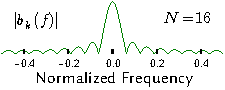
\includegraphics{wrapped_sinc}
  \end{columns}%
  \item Sample at discretized frequency point ${\color{blue}n\phi}$
  \item Integrate over delay window of discretized delay point ${\color{purple}p\tau}$
 \end{enumerate}
\end{frame}

\begin{frame}{Representing an off-grid point target}
 Off-grid point targets are still relatively sparse!
 \begin{itemize}
  \item All coefficients outside delay window $p_t$ are zero
  \item For frequency index, behavior dictated by wrapped sinc:
 \end{itemize}
 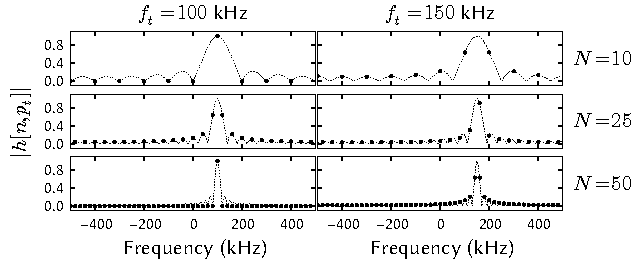
\includegraphics{point_target_coefficients}
 \begin{alertblock}{}
  Relative sparsity improves with increasing $N$\\(same number significant coefficients, many more zeros)
 \end{alertblock}
\end{frame}

\section{Sparsity Background}
\subsection{Compressed Sensing}

\begin{frame}{Under-determined systems of equations}
 Not enough measurements to constrain unknown values\\(e.g. the radar model):
 \vspace{1ex}
 \begin{columns}[onlytextwidth]
  \column{0.2\textwidth}
  \centering
  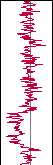
\includegraphics{head_and_flare_example_signal}
  \column{0.5\textwidth}
   $%\begin{equation*}
    {\color{purple}
    \begin{bmatrix}
     \\y\\\ 
    \end{bmatrix}}
    = 
    {\color{blue}
    \begin{bmatrix}
     &&&&&&\\
     &&&A&&&\\
     &&&&&&
    \end{bmatrix}}
    {\color{red}
    \begin{bmatrix}
     \\\\h\\\\\ 
    \end{bmatrix}}
   $%\end{equation*}
  \column{0.3\textwidth}
  \centering
  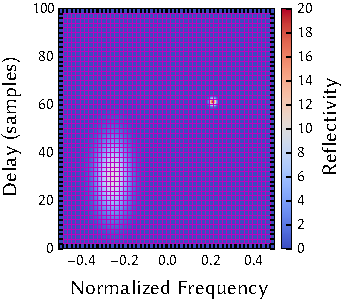
\includegraphics[width=\textwidth]{range_doppler_discretization}\\
  \textcolor{red}{(vectorized as $h$)}
 \end{columns}
 
 \begin{center}
  {\color{purple}Measurement}\hspace{3ex}{\color{blue}Model}\hspace{3ex}{\color{red}Unknown}\hspace*{9ex}
 \end{center}
 \begin{itemize}
  \item Infinite number of solutions
  \item Often know that the true solution should be sparse
  \item Finding the sparsest solution is hard in general
 \end{itemize}
\end{frame}

\begin{frame}{Theory of compressed sensing}
 \begin{definition}
  \alert{Compressed sensing} is a theory to guarantee solution of an under-determined set of equations.
 \end{definition}
 \begin{block}{Approximate guidelines for application}
  \begin{itemize}
   \item Solution known to be sparse
   \item Measurements are "incoherent" (global with low correlation)
   \item Minimum number of measurements on the order of the solution sparsity (number of nonzeros)
  \end{itemize}
 \end{block}
 \begin{block}{Benefit}
  Can solve easy convex optimization problem instead of hard combinatorial problem.
 \end{block}
\end{frame}

\begin{frame}{Equivalent convex optimization problem}
 \begin{block}{Sparsest solution to noisy measurements}
  \vspace{-2ex}
  \begin{align*}
   & \text{Find sparsest} && h\\
   & \text{subject to} && \norm{2}{y - A(h)} < \eta &&& \norm{2}{h}^2 =& \sum_k \abs{h_k}^2
  \end{align*}
  \vspace{-2ex}
 \end{block}
 \begin{block}{$l_1$-regularized least-squares (convex)}
  \vspace{-2ex}
  \begin{align*}
   & \underset{h}{\text{minimize}} && \frac{1}{2}\norm{2}{y - A(h)}^2 + \lambda\norm{1}{h} &&& \norm{1}{h} =& \sum_k \abs{h_k}
  \end{align*}
  \vspace{-2ex}
 \end{block}
 The $l_1$-norm promotes sparsity!
\end{frame}

\subsection{Convex Optimization}

\begin{frame}{First-order methods}
 We want to efficiently solve
 \begin{equation*}
  \underset{h}{\text{minimize}} \quad \frac{1}{2}\norm{2}{y - A(h)}^2 + \lambda\norm{1}{h}
 \end{equation*}
 but for systems $A$ that are too large for matrix methods.
 
 \begin{block}{First-order methods}
  \begin{itemize}
   \item Explicit matrix for $A$ not needed
   \item Only need to be able to compute $A(\cdotp)$ and $A^*(\cdotp)$
  \end{itemize}
 \end{block}
 
 \begin{alertblock}{}
  $l_1$-regularized least-squares is non-smooth because of the $l_1$ norm term, so minimizing it requires a special approach.
 \end{alertblock}
\end{frame}

\begin{frame}{First-order step}{Smooth}
 If the function being minimized is differentiable, the most natural first-order step is a gradient step.
 \begin{center}
  \movie[autostart,loop,width=4in,height=2in]{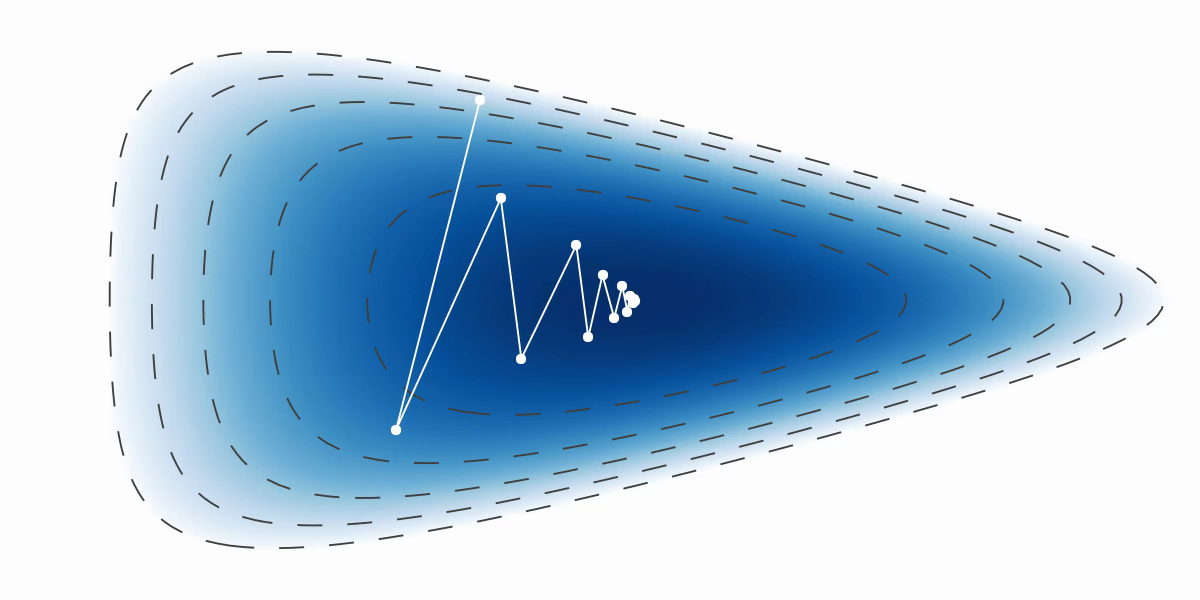
\includegraphics[width=4in]{gradient_descent_animation}}{movies/gradient_descent_animation.mp4}
 \end{center}
\end{frame}

\begin{frame}{First-order step}{Non-smooth}
 For a non-differentiable function, an attractive alternative is the proximal (or prox) step.
 \begin{equation*}
  x^{k+1} \coloneqq \argmin_{x} \; \left( {\color{purple}G(x)} + {\color{blue} \frac{1}{2\mu} \norm{2}{x - x^{k}}^2 } \right)
 \end{equation*}
 \begin{columns}[onlytextwidth]
  \column{0.33\textwidth}
  \column{0.33\textwidth}
  \centering
  {\color{purple}Non-smooth function}
  \column{0.33\textwidth}
  \centering
  {\color{blue}Smoothing around current iterate}
 \end{columns}
 \begin{itemize}
  \item This is surprisingly easy to solve and can be evaluated much like a gradient!
  \item Note that as $x^{k}$ approaches the minimum $x^*$, the smoothing term goes to zero.
 \end{itemize}
 The \alert{prox operator} is defined for non-smooth $G(x)$ as
 \begin{equation*}
  \mathbf{prox}_{\mu G} (v) = \argmin_{x} \; \left( G(x) + \frac{1}{2\mu} \norm{2}{x - v}^2 \right).
 \end{equation*}
\end{frame}

\begin{frame}{Proximal gradient method}
 The \alert{proximal gradient method} combines gradient and prox steps to solve
 \begin{equation*}
  \underset{x}{\text{minimize}} \quad F(x) + G(x)
 \end{equation*}
 for smooth $F(x)$ and non-smooth $G(x)$.
 \begin{block}{Algorithm}
  (Step size $\mu$) Iterate:
  \vspace{-2ex}
  \begin{align*}
   \text{Gradient step} && z^{k+1} &\coloneqq x^{k} - \mu \nabla F\left(x^{k}\right)\\
   \text{Prox step} && x^{k+1} &\coloneqq \mathbf{prox}_{\mu G}\left(z^{k+1}\right)
  \end{align*}
  \vspace{-2ex}
 \end{block}
\end{frame}

\begin{frame}<1>{Proximal gradient method applied}
 \begin{beamercolorbox}{example text}
  Proximal gradient for $l_1$-regularized least-squares:
 \end{beamercolorbox}
 \begin{equation*}
  \underset{h}{\text{minimize}} \quad \frac{1}{2}\norm{2}{y - A(h)}^2 + \lambda\norm{1}{h}
 \end{equation*}
 \begin{flalign*}
  &F(h) = \frac{1}{2}\norm{2}{y - A(h)}^2 \quad{\color{red}\Longrightarrow}\quad \nabla F(h) = -A^*\left(y - A(h)\right)\\
  &G(h) = \lambda\norm{1}{h} \quad{\color{red}\Longrightarrow}\quad
  \mathbf{prox}_{\mu G}(v) = \mathbf{soft}_{\lambda\mu}(v) = \begin{cases}
                              v - \lambda\mu, & v > \lambda\mu\\
                              0, & \abs{v} \le \lambda\mu\\
                              v + \lambda\mu, & v < -\lambda\mu
                             \end{cases}
 \end{flalign*}
 \only<2->{
 \begin{block}{Iterative Soft Thresholding}
  \vspace{-4ex}
  \begin{align*}
   \text{Matched filtering of error} && z^{k+1} &\coloneqq h^{k} + \mu A^*\left(y - A(h^{k})\right)\\
   \text{Soft thresholding} && h^{k+1} &\coloneqq \mathbf{soft}_{\lambda\mu}\left(z^{k+1}\right)
  \end{align*}
  \vspace{-3ex}
 \end{block}
 }
\end{frame}

\begin{frame}{Iterative Soft Thresholding}
 \begin{columns}
   \column{0.6\textwidth}
   \parbox[c][0.505in]{0.45\textwidth}{\raggedright Guess:}%
   \hspace{0.05\textwidth}%
   \parbox[c][0.505in]{0.5\textwidth}{$h$}\\
   \parbox[c][0.505in]{0.45\textwidth}{\raggedright Forward model, calculate error:}%
   \hspace{0.05\textwidth}%
   \parbox[c][0.505in]{0.5\textwidth}{$z = y - A(h)$}\\
   \parbox[c][0.505in]{0.45\textwidth}{\raggedright Matched filtering of error:}%
   \hspace{0.05\textwidth}%
   \parbox[c][0.505in]{0.5\textwidth}{$A^*(z)$}\\
   \parbox[c][0.505in]{0.45\textwidth}{\raggedright Add previous guess:}%
   \hspace{0.05\textwidth}%
   \parbox[c][0.505in]{0.5\textwidth}{$h + A^*(z)$}\\
   \parbox[c][0.505in]{0.45\textwidth}{\raggedright Threshold to form new guess:}%
   \hspace{0.05\textwidth}%
   \parbox[c][0.505in]{0.5\textwidth}{$h = \mathbf{soft}(h + A^*(z))$}\\
   \column{0.4\textwidth}
   \centering
   \movie[autostart,loop,width=1.8in,height=2.7in]{\includegraphics[width=1.8in]{ist_animation}}{movies/ist_animation.mp4}
 \end{columns}
\end{frame}

\section{Waveform Inversion}

\subsection{Implementation}

\begin{frame}{Combined algorithmic advances}
 First order prox algorithms are an active research area, so I tested and combined multiple proposed enhancements.
 \begin{columns}
  \column{0.5\textwidth}
   \begin{enumerate}
    \item Accelerated proximal gradient method
    \begin{itemize}
     \item Adds simple "momentum" term
     \item Better theoretical convergence
    \end{itemize}
    \item Adaptive restart
    \begin{itemize}
     \item Reset acceleration when it opposes prior step
    \end{itemize}
    \item Adaptive step size
    \begin{itemize}
     \item Increase step size every iteration
     \item Decrease as necessary to ensure convergence
    \end{itemize}
   \end{enumerate}

  \column{0.5\textwidth}
  \centering
  \begin{exampleblock}{Convergence comparison}
   \begin{tabular}{cc}
    Method & Iterations\\\hline
    Prox gradient & 4463\\
    + Acceleration & 2911\\
    + Adaptive restart & 397\\
    + Adaptive step & 105
   \end{tabular}
  \end{exampleblock}
 \end{columns}
\end{frame}

\begin{frame}{Testing similar algorithms}
 Other prox-based algorithms are worthy of consideration:
 \begin{itemize}
  \item Linearized alternating direction method of multipliers (ADMM)
  \item Primal-dual hybrid gradient (PDHG)
 \end{itemize}

 
 These both solve
 \begin{equation*}
  \underset{x}{\text{minimize}} \quad F(x) + G(x)
 \end{equation*}
 when both $F(x)$ and $G(x)$ can be non-smooth.
 \begin{exampleblock}{Convergence comparison}
  \centering
  \begin{tabular}{cc}
   Method & Iterations\\\hline
   Accelerated proximal gradient & 105\\
   Linearized ADMM (with adaptive step) & 154\\
   PDHG (fixed step) & 4464
  \end{tabular}
 \end{exampleblock}
\end{frame}

\begin{frame}{Code}
 Python/Cython/Numba
\end{frame}

\begin{frame}{Interpretation}
 Iterative thresholding matched filter
 Sparse solution to sidelobe removal
\end{frame}

\subsection{Experimental Results}

\begin{frame}{The Jicamarca incoherent scatter radar}
 \begin{columns}
  \column{0.5\textwidth}
  Specifications:
  \column{0.5\textwidth}
  Reasons:
 \end{columns}
 \begin{columns}
  \column{0.5\textwidth}
  \begin{itemize}
   \item Located outside Lima, Peru
   \item VHF (50 MHz)
   \item Phased array of 96 $\times$\ 96 crossed half-wave dipoles
   \includegraphics[height=0.6\textwidth]{jicamarca}
   \item 1 MHz bandwidth (TX/RX)
  \end{itemize}
  \column{0.5\textwidth}
  \begin{itemize}
   \item Equatorial ionosphere is challenging\\
   \includegraphics[width=0.9\textwidth]{equatorial_example_mf_rti_3}
   \item Detection rate of meteors is better at lower frequencies
   \item Interferometry and/or dual polarization receive
  \end{itemize}
 \end{columns}
\end{frame}

\begin{frame}{Jicamarca experiment goals}
 \begin{columns}
  \column{0.4\textwidth}
  \begin{block}{Goals}
   \begin{itemize}
    \item Test sparsity-based waveform inversion in \alert{crowded environment}
    \item Directly compare effectiveness of different waveforms
   \end{itemize}
  \end{block}
  \column{0.6\textwidth}
  \centering
  \includegraphics{ejet_head_flare_mf_rti_3}
 \end{columns}
\end{frame}

\begin{frame}{Jicamarca meteor experiment}
 \begin{columns}
  \column{0.55\textwidth}
  \begin{block}{Description}
   Alternating sequence of 5 common waveforms for observing meteor region (80-140 km altitude).
  \end{block}
  \column{0.46\textwidth}
  \begin{block}{Parameters}
   \vspace{-1.25ex}
   \begin{itemize}
    \item Pulse interval of 1 ms
    \item Sample time of 1 $\mu$s\\(150 m range resolution)
   \end{itemize}
   \vspace{-1.25ex}
  \end{block}
 \end{columns}
 \vspace{2ex}
 \includegraphics{head_and_flare_mf_rti_block}
\end{frame}

\begin{frame}{Movie of meteor sidelobe removal}
 \movie[autostart,loop,width=4.320687in,height=2.28in]{\includegraphics[width=4.320687in]{head_and_flare_mf_vs_recovered_1}}{movies/head_and_flare_mf_vs_recovered_1.mp4}
\end{frame}

\begin{frame}[t]{Example: Minimum sidelobe code}
 \begin{tikzpicture}
  \tikzstyle{every node}=[minimum width=\widthof{Waveform}+2ex]
  \node[left,align=center] at (0,0.5) {Matched\\Filter};
  \node[right,image] at (0,0) {\includegraphics{head_and_flare_mf_rti_1}};
  \fill[white] (0,-1.125) rectangle (9,-0.875);
  \node[left,align=center] at (0,-2.3) {Waveform\\Inversion};
  \node[right,image] at (0,-2.8) {\includegraphics{head_and_flare_recovered_rti_noise_1}};
 \end{tikzpicture}
\end{frame}

\begin{frame}[t]{Example: Barker-13 code}
 \begin{tikzpicture}
  \tikzstyle{every node}=[minimum width=\widthof{Waveform}+2ex]
  \node[left,align=center] at (0,0.5) {Matched\\Filter};
  \node[right,image] at (0,0) {\includegraphics{head_and_flare_mf_rti_0}};
  \fill[white] (0,-1.125) rectangle (9,-0.875);
  \node[left,align=center] at (0,-2.3) {Waveform\\Inversion};
  \node[right,image] at (0,-2.8) {\includegraphics{head_and_flare_recovered_rti_noise_0}};
 \end{tikzpicture}
\end{frame}

\begin{frame}[t]{Example: Pseudorandom code}
 \begin{tikzpicture}
  \tikzstyle{every node}=[minimum width=\widthof{Waveform}+2ex]
  \node[left,align=center] at (0,0.5) {Matched\\Filter};
  \node[right,image] at (0,0) {\includegraphics{head_and_flare_mf_rti_4}};
  \fill[white] (0,-1.125) rectangle (9,-0.875);
  \node[left,align=center] at (0,-2.3) {Waveform\\Inversion};
  \node[right,image] at (0,-2.8) {\includegraphics{head_and_flare_recovered_rti_noise_4}};
 \end{tikzpicture}
 \vspace{-5ex}
 \begin{alertblock}{}<2>
  Works with variety of codes
 \end{alertblock}
\end{frame}

\begin{frame}[t]{Example: LFM chirp}
 \begin{tikzpicture}
  \tikzstyle{every node}=[minimum width=\widthof{Waveform}+2ex]
  \node[left,align=center] at (0,0.5) {Matched\\Filter};
  \node[right,image] at (0,0) {\includegraphics{head_and_flare_mf_rti_3}};
  \fill[white] (0,-1.125) rectangle (9,-0.875);
  \node[left,align=center] at (0,-2.3) {Waveform\\Inversion};
  \node[right,image] at (0,-2.8) {\includegraphics{head_and_flare_recovered_rti_noise_3}};
 \end{tikzpicture}
 \vspace{-5ex}
 \begin{alertblock}{}<2>
  Some codes are troublesome
 \end{alertblock}
\end{frame}

\begin{frame}[t]{Example: Uncoded}
 \begin{tikzpicture}
  \tikzstyle{every node}=[minimum width=\widthof{Waveform}+2ex]
  \node[left,align=center] at (0,0.5) {Matched\\Filter};
  \node[right,image] at (0,0) {\includegraphics{head_and_flare_mf_rti_2}};
  \fill[white] (0,-1.125) rectangle (9,-0.875);
  \node[left,align=center] at (0,-2.3) {Waveform\\Inversion};
  \node[right,image] at (0,-2.8) {\includegraphics{head_and_flare_recovered_rti_noise_2}};
 \end{tikzpicture}
 \vspace{-5ex}
 \begin{alertblock}{}<2>
  Works even with uncoded pulses!
 \end{alertblock}
\end{frame}

\begin{frame}[t]{Waveform inversion code comparison}
 \begin{tikzpicture}
  \tikzstyle{every node}=[minimum width=\widthof{Waveform}+2ex]
  \node<1>[left,align=center] at (0,0.5) {Minimum\\sidelobe};
  \node<1>[right,image] at (0,0) {\includegraphics{head_and_flare_recovered_rti_noise_1}};
  \node<2->[left,align=center] at (0,0.5) {Pseudo-\\random};
  \node<2->[right,image] at (0,0) {\includegraphics{head_and_flare_recovered_rti_noise_4}};
  \fill[white] (0,-1.125) rectangle (9,-0.875);
  \node[left,align=center] at (0,-2.3) {Uncoded};
  \node[right,image] at (0,-2.8) {\includegraphics{head_and_flare_recovered_rti_noise_2}};
 \end{tikzpicture}
 \vspace{-5ex}
 \begin{alertblock}{}<3->
  Quality of solution depends on fidelity of waveform
 \end{alertblock}
\end{frame}

\section{Conclusion}

\begin{frame}<beamer>{Outline}
 \tableofcontents[currentsection,hideallsubsections]
\end{frame}

\begin{frame}{Benefits of waveform inversion}
 \begin{columns}
  \column{0.5\textwidth}
  \begin{enumerate}
   \item \alert{Sidelobe removal} -\\
   Removes ambiguity for observation of multiple or range-spread targets\\
   (e.g. fragmentation and non-specular trails)
   \item \alert{Full frequency decoding} -\\
   Decodes over full frequency spectrum simultaneously, for target differentiation in crowded environments\\
   (e.g. equatorial, flares)
   \item \alert{Flexibility} -\\
   Enables use of many different waveforms
  \end{enumerate}
 \column{0.5\textwidth}
 \includegraphics[width=\textwidth]{mathews_fragmentation}\\
 \includegraphics[width=\textwidth]{head_and_flare_mf_rti_3}\\
 \includegraphics[width=\textwidth]{equatorial_example_mf_rti_3}
 \end{columns}
\end{frame}

\againframe<7->{contributions}

\begin{frame}{Further research}
 \begin{block}{Near-universal radar measurements}
  Submitted NSF postdoc proposal to work at MIT Haystack (Millstone Hill) and create near-universal measurement mode across radar chain using uniquely-tuned waveforms.
 \end{block}
 \begin{block}{Self-calibration}
  Iteratively solve for reflectivity \emph{and} transmitted waveform to better characterized the radar system.
 \end{block}
 \begin{block}{Passive radar}
  Waveform flexibility invites use for parasitic radio science (using FM radio, digital TV signals) where the transmitted waveform cannot be controlled.
 \end{block}
\end{frame}

\begin{frame}{Acknowledgements}
 
\end{frame}

\begin{frame}{Questions}
 \tableofcontents
\end{frame}

\appendix

% \begin{frame}{Classical detection with the matched filter}
%  \begin{block}{Ideal point target}
%   \begin{itemize}
%    \item Point target perfectly reflects the transmitted signal
%    \item Receive attenuated copy of signal after some delay
%    \item Delay is a function of the target's range
%   \end{itemize}
%  \end{block}
%  \begin{block}{Matched filter properties}
%   \begin{itemize}
%    \item Peak of output gives \alert{maximum likelihood estimate} of target's range and amount of attenuation
%    \item Maximum signal-to-noise ratio (SNR) at peak of all filters
%   \end{itemize}
%  \end{block}
% \end{frame}

% \begin{frame}{Ambiguity between measurement and target}
%  
% \end{frame}

% \begin{frame}{Radar model assumptions}
%  
% \end{frame}

% \begin{frame}{Towards ambiguity inversion}
%  \begin{block}{Ambiguity equation}
%   Represent matched filter ambiguity as linear system $X$:
%   \begin{equation*}
%    x[n,p] = X\left(h[n,p]\right) \quad\longrightarrow \text{Equation is non-invertible.}
%   \end{equation*}
%  \end{block}
%  \begin{block}{Make matched filtering explicit}
%   Let $A^*$ represent frequency-shifted matched filtering. Then
%   \begin{equation*}
%    X(h) = A^*\left(A(h)\right)
%   \end{equation*}
%   the ambiguity operation is matched filtering composed with its adjoint. Rewrite the ambiguity equation:
%   \begin{equation*}
%    A^*\left(y[m]\right) = A^*\left(A\left(h[n,p]\right)\right)
%   \end{equation*}
%  \end{block}
% \end{frame}
% 
% \begin{frame}{Sparsity of non-point targets}
%  We have the exact equation:
%  \begin{block}{Reflectivity coefficient equation}
%   \vspace{-2ex}
%   \begin{equation*}
%    h[n,p] = \int_{p \tau}^{(p+1)\tau} \left[h(f, \lambda) e^{2\pi i f \lambda} * b_{p + 1}(f) \right](n\Delta{f}) \dee\lambda
%   \end{equation*}
%   \vspace{-2ex}
%  \end{block}
%  \begin{itemize}
%   \item Blurring from wrapped sinc mostly preserves sparsity (evidenced by point target analysis)
%   \item Integration over delay exactly preserves sparsity
%  \end{itemize}
%  \begin{alertblock}{}
%   If a target has a sparse reflectivity function, we can reasonably expect its reflectivity coefficient representation to be sparse as well.
%  \end{alertblock}
% \end{frame}
% 
% \begin{frame}{The prox operator}
%  The proximal operator, or \alert{prox operator}, is defined for non-smooth $G(x)$ as
%  \begin{equation*}
%   \mathbf{prox}_{\mu G} (v) = \argmin_{x} \; \left( G(x) + \frac{1}{2\mu} \norm{2}{x - v}^2 \right).
%  \end{equation*}
%  \begin{exampleblock}{Projection onto a set}
%   If $G(x)$ is the indicator function for a closed convex set $\mathcal{C}$,
%   \begin{equation*}
%    G(x) = \begin{cases}
%            0 & x \in \mathcal{C}\\
%            \infty & x \notin \mathcal{C}
%           \end{cases}
%   \end{equation*}
%   $\mathbf{prox}_{G}(v)$ is projection of $v$ onto $\mathcal{C}$.
%  \end{exampleblock}
% \end{frame}

% \begin{frame}{Linearized ADMM}
%  
% \end{frame}

% \begin{frame}{Accelerated proximal gradient method}
%  
% \end{frame}

% \subsection{Implementation}
%
% Why prox algorithms?
% 
% \begin{frame}{FISTA with radar model}
%  Compute model with FFTW and Cython\\
%  Adaptive step size
% \end{frame}
% 
% \begin{frame}{Waveform inversion}
%  l1-rls gives sparse solution\\
%  Leaves unmodeled noise\\
%  Matched filter the unmodeled noise\\
%  Add noise back to sparse solution = sidelobe removal\\
%  Ambiguity function is $A^*A$, so sidelobes are $(A^*A - I)$
% \end{frame}
% 
% \begin{frame}{Sparse solution}
%  delay-frequency figure
% \end{frame}
% 
% \begin{frame}{Unmodeled noise}
%  delay-frequency figure
% \end{frame}
% 
% \begin{frame}{Sidelobe removal}
%  delay-frequency figure
% \end{frame}

\end{document}
